% SMS LaTeX Thesis Template
% Sensory-Motor Systems Lab
% Swiss Federal Institute of Technology (ETH) Zurich
%
% ---------------------------------------------------------------------------------------------------------------
% This Template is based on the IMRT LaTex Template by Eric Mueller (2004) and Soren 
% Ebbesen (2013).
% ---------------------------------------------------------------------------------------------------------------
%
% Revisions: 	2013-06-18  (Nicolas Gerig)
% ______________________________________________________________________________
\documentclass[10pt,twoside,a4paper,fleqn]{report}

\usepackage[english,st,nobalgrist]{ethsms} % Special IDSC styles and commands      	
								 % {german}/english: language of headings, etc.
								 % {st}/bt/mt: {semester}/bachelor/master thesis
								 % {balgrist}/nobalgrist: {include Balgrist Logos}/exclude Balgrist Logos
							

% Title page (please fill in)___________________________________________________
\title{Evaluation of Master Devices for TAVI/TAVR Teleoperated Robot}


\studentA{Armando Daniel Amoros Lozano}
\ethidA{17-940-248}
\semesterA{5}
\emailA{aarmando@student.ethz.ch}

%\studentB{Second Student}
%\ethidB{12-345-678}
%\semesterB{9}
%\emailB{second@student.ethz.ch}

\supervision{Prof. Dr. Robert Riener\\PD Dr. med. Andre Plass Leitender}
\date{October 2019}

% Begin document________________________________________________________________
\begin{document}

\maketitle 							% Create title page

% Page headers (don't change)____________________________________________________
\pagestyle{fancy}               	% Fancy headings

% Preamble______________________________________________________________________
\pagenumbering{roman} 				% Begin roman page numbering (i,ii,...)

%Die übersicht sollte in englischer und in deutscher Sprache verfasst werden
%the abstract should include an english and a german version
% !TeX root = /../Report.tex

\chapter*{Abstract\markboth{Abstract}{Abstract}}
\addcontentsline{toc}{chapter}{\protect\numberline{}Abstract}
\label{abstract}

This thesis work intends to find the most suitable master device type for a TAVI/TAVR teleoperated robot, capable of controlling the 2 DOF (translation and rotation) of the different catheters and guide wires used during the intervention.\\

After a state-of-the-art research in catheter handling teleoperated robots, four different master devices were tested, each device controls each one of the 2 DOF independently. The first device with completely digital inputs (Keyboard type), the second device hybrid with 1 digital input (translation) and 1 analogical input (rotation) (Remote Controller type), and the remaining two devices with completely analogical inputs (Joystick type and CatheterLike type).\\

The experiments were performed by 15 candidates from which 1 was an expert TAVI surgeon. Each device was tested under three different experiments and by the appreciation of the users, the first two experiments were designed as a follow the target task assessing the precision and response of each DOF independently. The third experiment was designed as a navigation task, using both DOF, measuring the time and smoothness of the movements and path followed until reaching the goal.\\

The results of the experiments and the user's poll responses indicate that the Joystick type device has a better overall performance for controlling the 2 DOF of a regular catheter used in TAVI/TAVR surgery.\\

\cleardoublepage

%Danksagungen
%acknowledgements
% !TeX root = /../Report.tex

\chapter*{Acknowledgements\markboth{Acknowledgements}{Acknowledgements}}
\addcontentsline{toc}{chapter}{\protect\numberline{}Acknowledgements}

%Put your acknowledgements in here.

% remove placeholder text START
I want to thank all the people, family and friends, that supported me one way or another before and during the course of my masters. Special thanks to Joaquin Campos, that supported my academic way even before this journey started, to my brothers and parents that have been there to support me even from far away whenever I needed it. Finally, special thanks to Tanya, Claudia and Roland Hansalik, for been the family I needed in Switzerland. 
% remove placeholder text END
\cleardoublepage

%Declaration of Originality
%Eigenständigkeitserklärung
\createDeclaration
\cleardoublepage

%Symbole
%symbols
% !TeX root = /../Report.tex

\chapter*{Symbols\markboth{Symbols}{Symbols}}\label{chap:symbols}
\addcontentsline{toc}{chapter}{\protect\numberline{}Symbols}

\section*{Symbols}
\begin{tabbing}
 \hspace*{3cm} \= \kill
  $m$							\> mass [kg] \\[0.5ex]
  $g$							\> gravitational acceleration [$m/s^2$] \\[0.5ex]  
  $\rho$ 						\> density [kg/m$^3$] \\[0.5ex]
 \end{tabbing}

\section*{Acronyms and Abbreviations}
\begin{tabbing}
 \hspace*{1.6cm}  \= \kill
 DNA \> Deoxyribonucleic acid \\[0.5ex]
 LED \> Light emitting diode \\[0.5ex]
 ETH \> Swiss Federal Institute of Technology \\[0.5ex]
 SMS	\> Sensory-Motor Systems Lab  \\[0.5ex]
\end{tabbing}
\cleardoublepage

%
\tableofcontents
\cleardoublepage
%
\listoffigures
\cleardoublepage


% Chapters______________________________________________________________________
\pagenumbering{arabic}				% Begin arabic page numbering (1,2,...)

% !TeX root = /../Report.tex

\chapter{Introduction}\label{sec:introduction}
This template is meant to be used for semester, bachelor, and master theses written at the Sensory-Motor Systems Lab (SMS), ETH Zurich. The template includes several examples of equations, figures, tables, etc. in order to act as a {\it very} short introduction to \TeX\! and \LaTeX. Yet, the template is also provided to ensure that all written work in \LaTeX ~at SMS shares identical formatting.
This template is based on the IMRT\footnote{Institute for Dynamic Systems and Control, ETH Zurich; www.imrt.ethz.ch} \LaTeX ~template by Eric Mueller (2009) and Soren Ebbesen (2013).

\section{The Preamble}\label{sec:preamble}
The preamble of the \LaTeX\! template defines the font size, page layout, language, report type, title, and author(s) of the report. The preamble of the current template is shown below. It should be more or less clear how you need to modify the preamble to fit your needs; if not, consult your supervisor.
%\lstset{language=TeX,numbers=none}
%\begin{lstlisting}[frame=lines]
\begin{verbatim}
\documentclass[10pt,twoside,a4paper,fleqn]{report}

\usepackage[english,st,balgrist]{ethsms} % Special SMS styles and commands      	
								 % {german}/english: language of headings, etc.
								 % {st}/bt/mt: {semester}/bachelor/master thesis
								 % {balgrist}/nobalgrist: {include Balgrist Logos}/exclude Balgrist Logos
							

% Title page (please fill in)___________________________________________________
\title{SMS \LaTeX\ Thesis Template v.1.0}


\studentA{Hans Muster}
\ethidA{97-906-739}
\semesterA{5}
\emailA{muster@student.ethz.ch}

%\studentB{Second Student}
%\ethidB{12-345-678}
%\semesterB{9}
%\emailB{second@student.ethz.ch}

\supervision{First Supervisor\\ Second Supervisor}
\date{March 2011}
 \end{verbatim}
%\end{lstlisting}

The style \texttt{ethsms.sty} enforces certain changes to the original \texttt{report} class, e.g., the title page. The style accepts three options. The first option lets you choose the language of your report, i.e., the language of the title page, headings, info-page, etc. Valid options are: \texttt{german} (default) and \texttt{english}. The second option defines the type of report which will be printed on the title and info page. Valid options are: \texttt{st} (default), \texttt{bt}, and \texttt{mt} for semester, bachelor and master thesis, respectively. The third option is to decide which logo configuration you will have on your title page.
Valid options are:  \texttt{balgrist} (default) and  \texttt{nobalgrist}, with this option you can choose to either include the UZH and Balgrist logos or not.
For instance, if you will be writing a master thesis in English and wish to add the UZH and Balgrist Logos, use
\begin{verbatim}
 \usepackage[english,mt,balgrist]{ethsms}
\end{verbatim}



\section{Compiling With pdfLatex}\label{sec:pdfLatex}

Some packages (pstricks) used for this template do need to be compiled to from latex to dvi to pdf.
If you want to use ''pdfLatex'' (as I do), then you need an additional setting to allow your compiler (for me it is Miktex on Windows) to create some ``in-between'' files and access them afterwards.

For TexWorks the required additional setting is shown in figure~\ref{img:pdfTexWorks}.
If you use the combination of ''pdfLatex+MakeIndex+BibTex'' the setting is slightly different, see figure~\ref{img:pdfTexWorks2}.

For other platforms and/or editors you can find information here: 

\url{http://tug.org/PSTricks/main.cgi?file=pdf/pdfoutput#texworks}

\begin{figure}[ht]
   \centering
   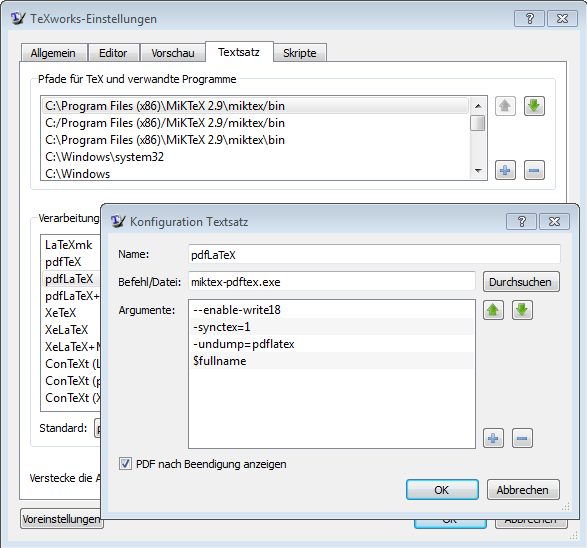
\includegraphics[width=0.9\textwidth]{img/pdfLatexSettingsForTexWorks.PNG}
   \caption{pdfLatex Settings in TexWorks}
   \label{img:pdfTexWorks}
\end{figure}

\begin{figure}[ht]
   \centering
   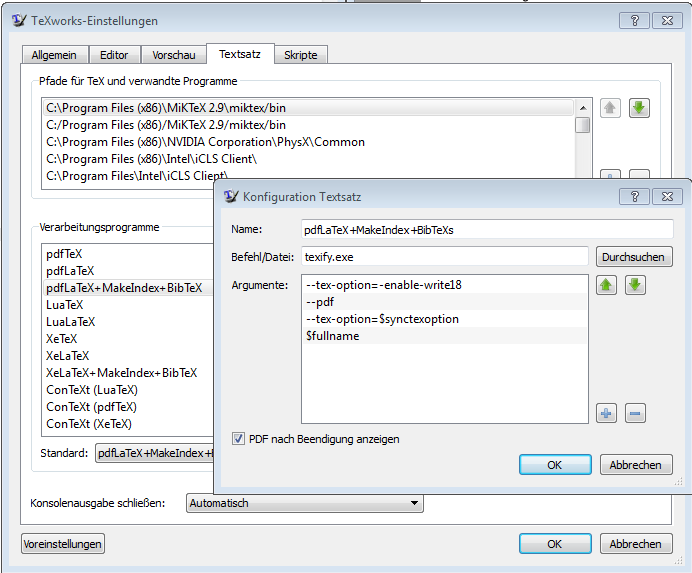
\includegraphics[width=0.9\textwidth]{img/pdfLatexMakeIndexBibTexSettingsForTexWorks.PNG}
   \caption{pdfLatex+MakeIndex+BibTex Settings in TexWorks}
   \label{img:pdfTexWorks2}
\end{figure}
\cleardoublepage
% !TeX root = /../Report.tex

\chapter{State of the art }\label{sec:stateoftheart}

Teleoperated robots for similar types of surgeries as TAVI have been developed. Figure~\ref{img:statetable} presents the robot's characteristics, such as the type of catheter they handle, the kind of intervention they were created for and the kind of master slave they operate with. On the other side figure~\ref{img:statedevices} shows the pictures of the master devices.\\

Devices like Niobe~\cite{stereoaxis} and Monarch~\cite{monarch} are highly costly and complex (much more than needed for a TAVI intervention, not mentioning that TAVI catheters could not be operated by Niobe magnetic fields, since they are plastic); on the other hand The Amigo system was designed to overcome these points having a simpler and cheaper designs~\cite{amigo}. Nevertheless, all these systems are designed to operate steerable catheters with 3 or more DOF, which make them an overkill for TAVI surgery, however, the concept behind their robotic devices could be simplified and adapted to only manage the 2 DOF necessary for TAVI.\\

Moreover, the CorPath GRX~\cite{corepath} is the system with the most similarities to what is needed for TAVI, handling 2 DOF catheters, guide wires and a stent balloon. However, TAVI surgery requires more than one catheter and guide wire to gain access to the left ventricle of the heart, as well as managing the new aortic valve deployer catheter.\\

These differences in characteristics and needs are the reason the devices in section~\ref{chosenDevices} where selected, taking into account the inherent research and effort the devices of the state of the art suppose, some of them were just simplified enough to cover TAVI surgery needs.\\

\begin{figure}[ht]
   \centering
   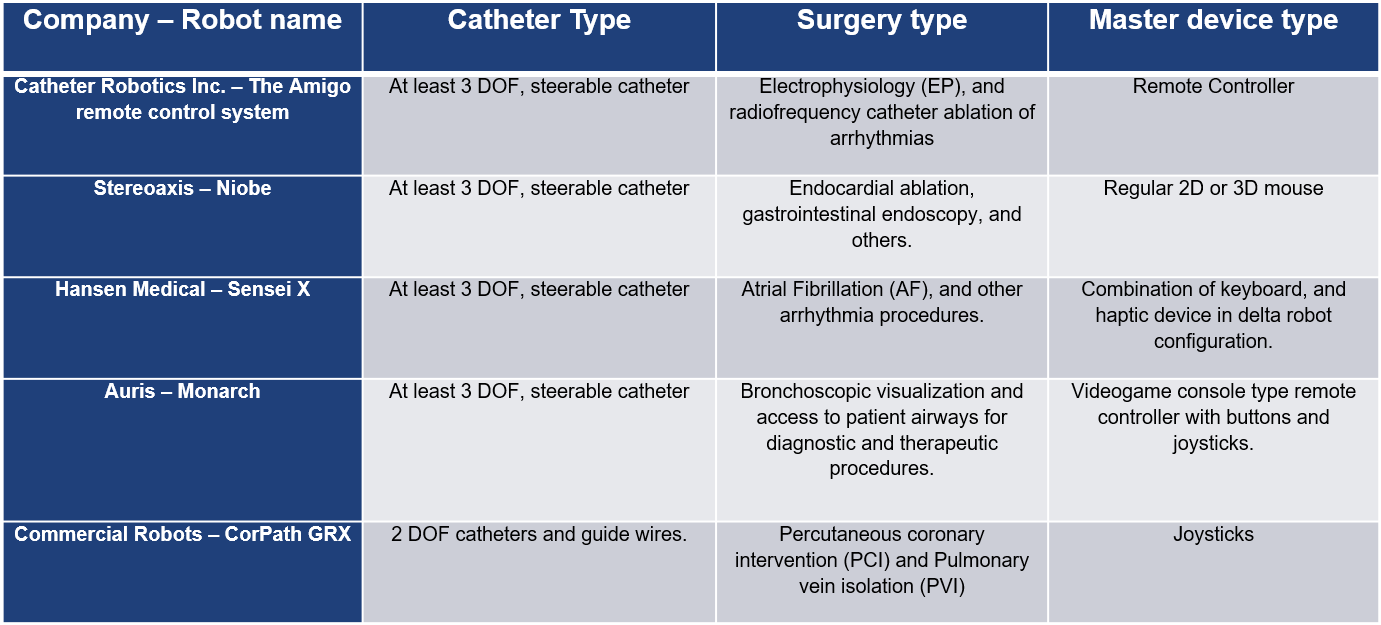
\includegraphics[width=1.0\textwidth]{img/statetable.PNG}
   \caption{Comparison between the state of the art devices in catheter teleoperation}
   \label{img:statetable}
\end{figure}

\begin{figure}[ht]
   \centering
   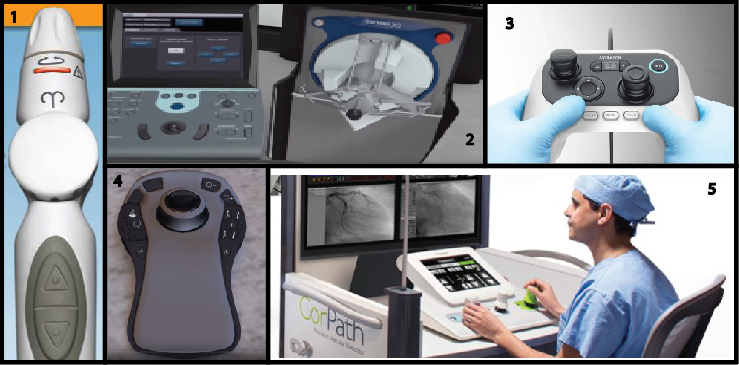
\includegraphics[width=1.0\textwidth]{img/statedevices.PNG}
   \caption{State of the art devices, (1) The Amigo Remote System, (2) Sensei X, (3) Monarch, (4) Stereoaxis and (5) CorPath GRX}
   \label{img:statedevices}
\end{figure}



\cleardoublepage
% !TeX root = /../Report.tex

\chapter{Chosen Master Devices and Characteristics}\label{chosenDevices}
Every device was chosen to control independently each one of the catheters DOF as shown in figure~\ref{img:dofi}. In this section the mechanics, electronics and functioning of every input device is explained. After, a comparison between all device's characteristics, advantages and disadvantages is made.

\begin{figure}[ht]
   \centering
   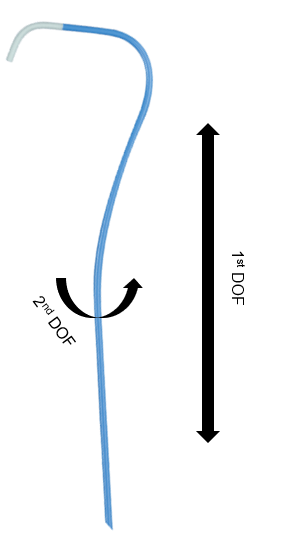
\includegraphics[width=0.4\textwidth]{img/Dof.PNG}
   \caption{TAVI catheter degrees of freedom}
   \label{img:dofi}
\end{figure}

\section{Keyboard}\label{sec:keyboard}
The keyboard device intends to represent any other device only controlled by on-off buttons, working in a digital configuration. For this experiment a numerical keypad was used figure~\ref{img:keyboardimg}.\\

The control of the catheter was performed with the arrow key, being the UP and Down arrow key the control for the 1st DOF of the catheter. The 2nd DOF was controlled with the RIGHT and LEFT arrow keys.\\

Both types of movements are mapped to the simulated catheter with a PressedTime-Velocity mapping. For information about the mapping refer to section~\ref{sec:mapping}.\\

\begin{figure}[ht]
   \centering
   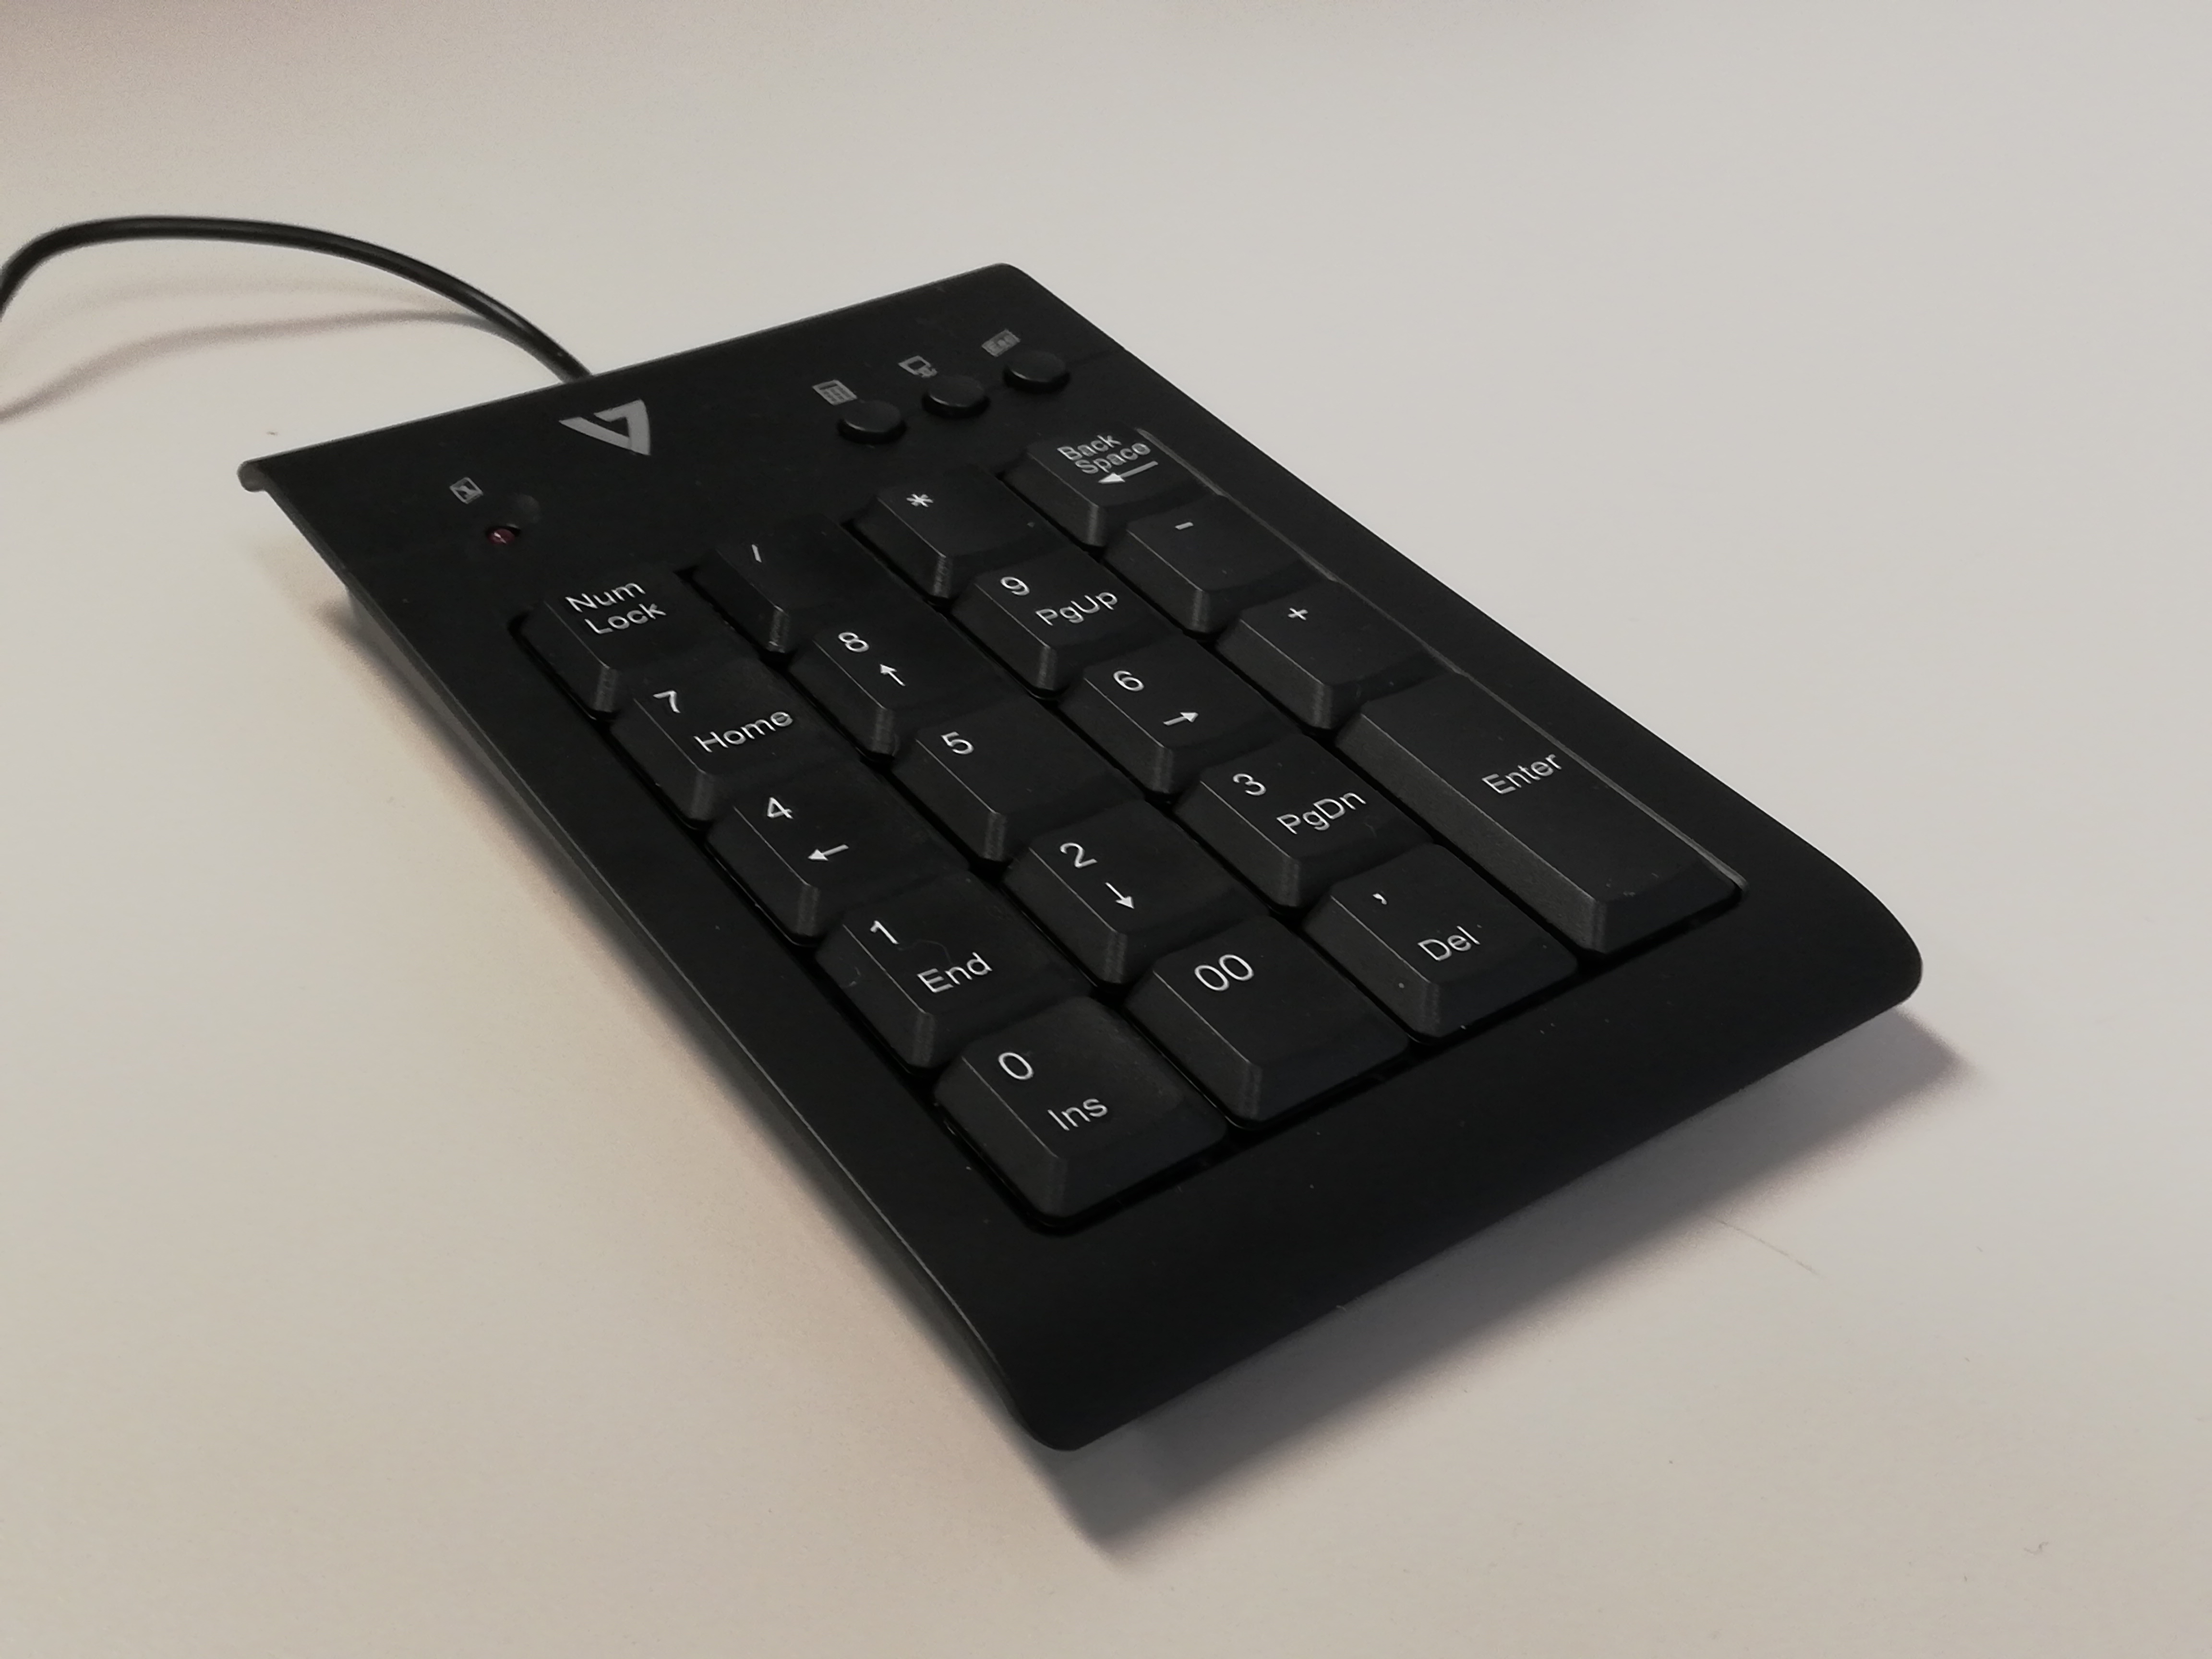
\includegraphics[width=0.7\textwidth]{img/keyboard.jpg}
   \caption{Keypad model V7-KP1019-USB-4EB with USB connection}
   \label{img:keyboardimg}
\end{figure}

\section{Remote}\label{sec:remote}
The Remote device is a combination of on-off buttons and a semi-analogical sensor figure~\ref{img:remotecad} and~\ref{img:remotenorm}. The shell of the device was 3D printed in ABS. Also equipped with two push buttons, and a continuous 360 degrees rolling disk.\\

The 1st DOF of the catheter is controlled using the two push buttons in a digital configuration. Movements in this DOF are mapped to the simulated catheter with a PressedTime-Velocity mapping.\\

The 2nd DOF is controlled by a non-contacting rotatory position sensor attached to the rolling disk, which gives a semi-analogical reading with a 12 BIT resolution per 360 degrees, this means. It Is important to notice that the experiment setup as can be seen in section~\ref{sec:arddevinter} uses an Arduino with a 10BIT ADC channel, which trims the initial sensor's 12BIT resolution. Movements in this DOF are mapped suing a Velocity-Velocity mapping.\\

For information about the mapping refer to section~\ref{sec:mapping}.\\

\begin{figure}[ht]
   \centering
   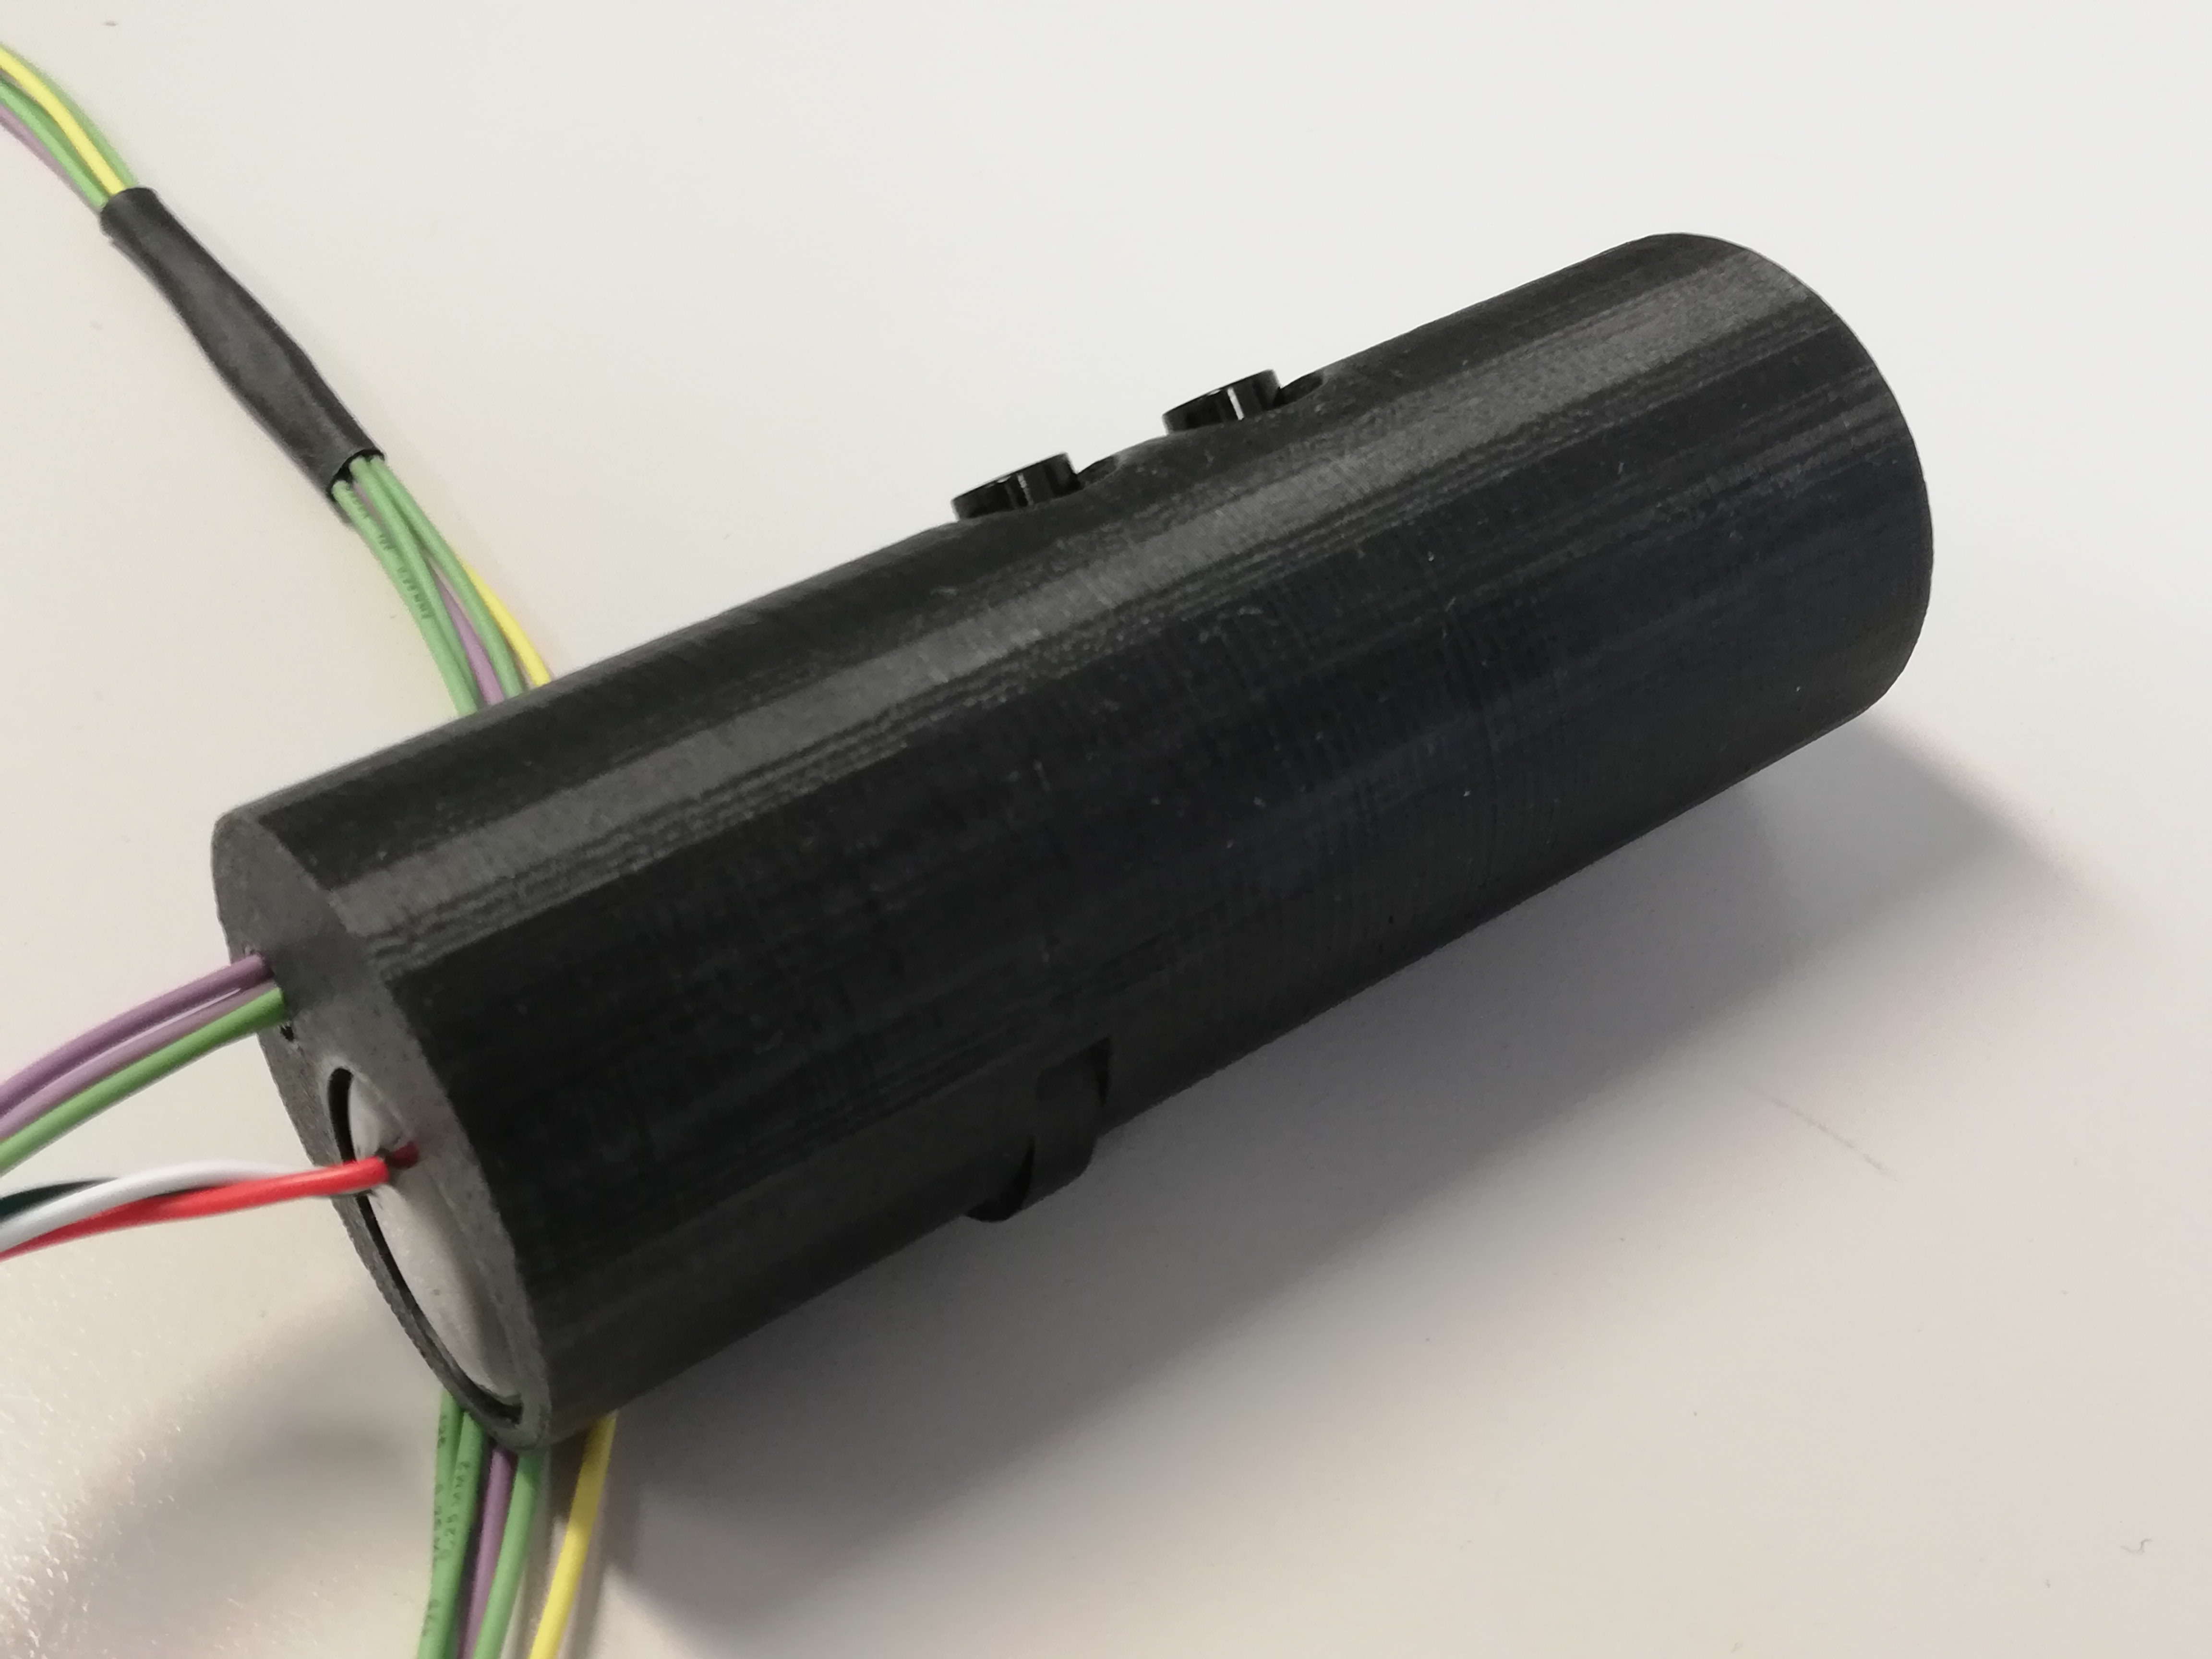
\includegraphics[width=0.7\linewidth]{img/remote.jpg}
   \caption{Remote device used for the experiments}
   \label{img:remotenorm}
\end{figure}

\begin{figure}[ht]
   \centering
   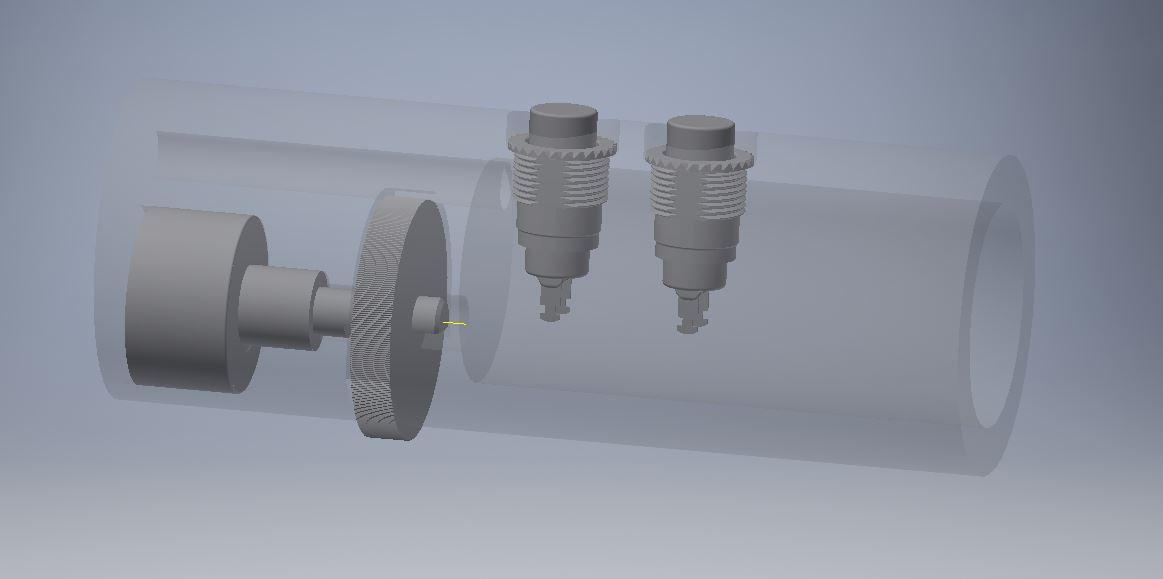
\includegraphics[width=0.7\linewidth]{img/remotecad.jpg}
   \caption{CAD design of the remote device, (push buttons C\&K 8532T1ZBE2) (Rotatory sensor CTS 285CCDFSAAB4C1)}
   \label{img:remotecad}
\end{figure}

\section{Joystick}\label{sec:joystick}

The Joystick device is implemented with fully with analogical sensors figure~\ref{img:joystickimg}. Originally the Joystick has 3 DOF available, plus a push button on the top. The roll DOF and the button are not connected at all. Thus, performing any movement on them will not make any difference in the outputs.\\

The 1st DOF of the catheter is controlled by a regular 5Kohm potentiometer, mapped on the pitch movement of the joystick. The movements in this DOF are translated to the simulation catheter with a Distance-Velocity mapping.\\

The 2nd DOF is also controlled by regular 5Kohm potentiometer mapped to the yaw movement of the joystick.\\

Both used DOF, pitch and yaw, are limited on their angle and brought back automatically to initial position by springs once any force is applied. The movements in both DOF are translated into the simulated catheter with a Position-Velocity mapping. For information about the mapping refer to section~\ref{sec:mapping}. \\

The potentiometers have essentially infinite resolution, only trimmed by the Arduino's ADC channel (See section~\ref{sec:arddevinter} for experiment setup) used to read out the sensors.\\

\begin{figure}[ht]
   \centering
   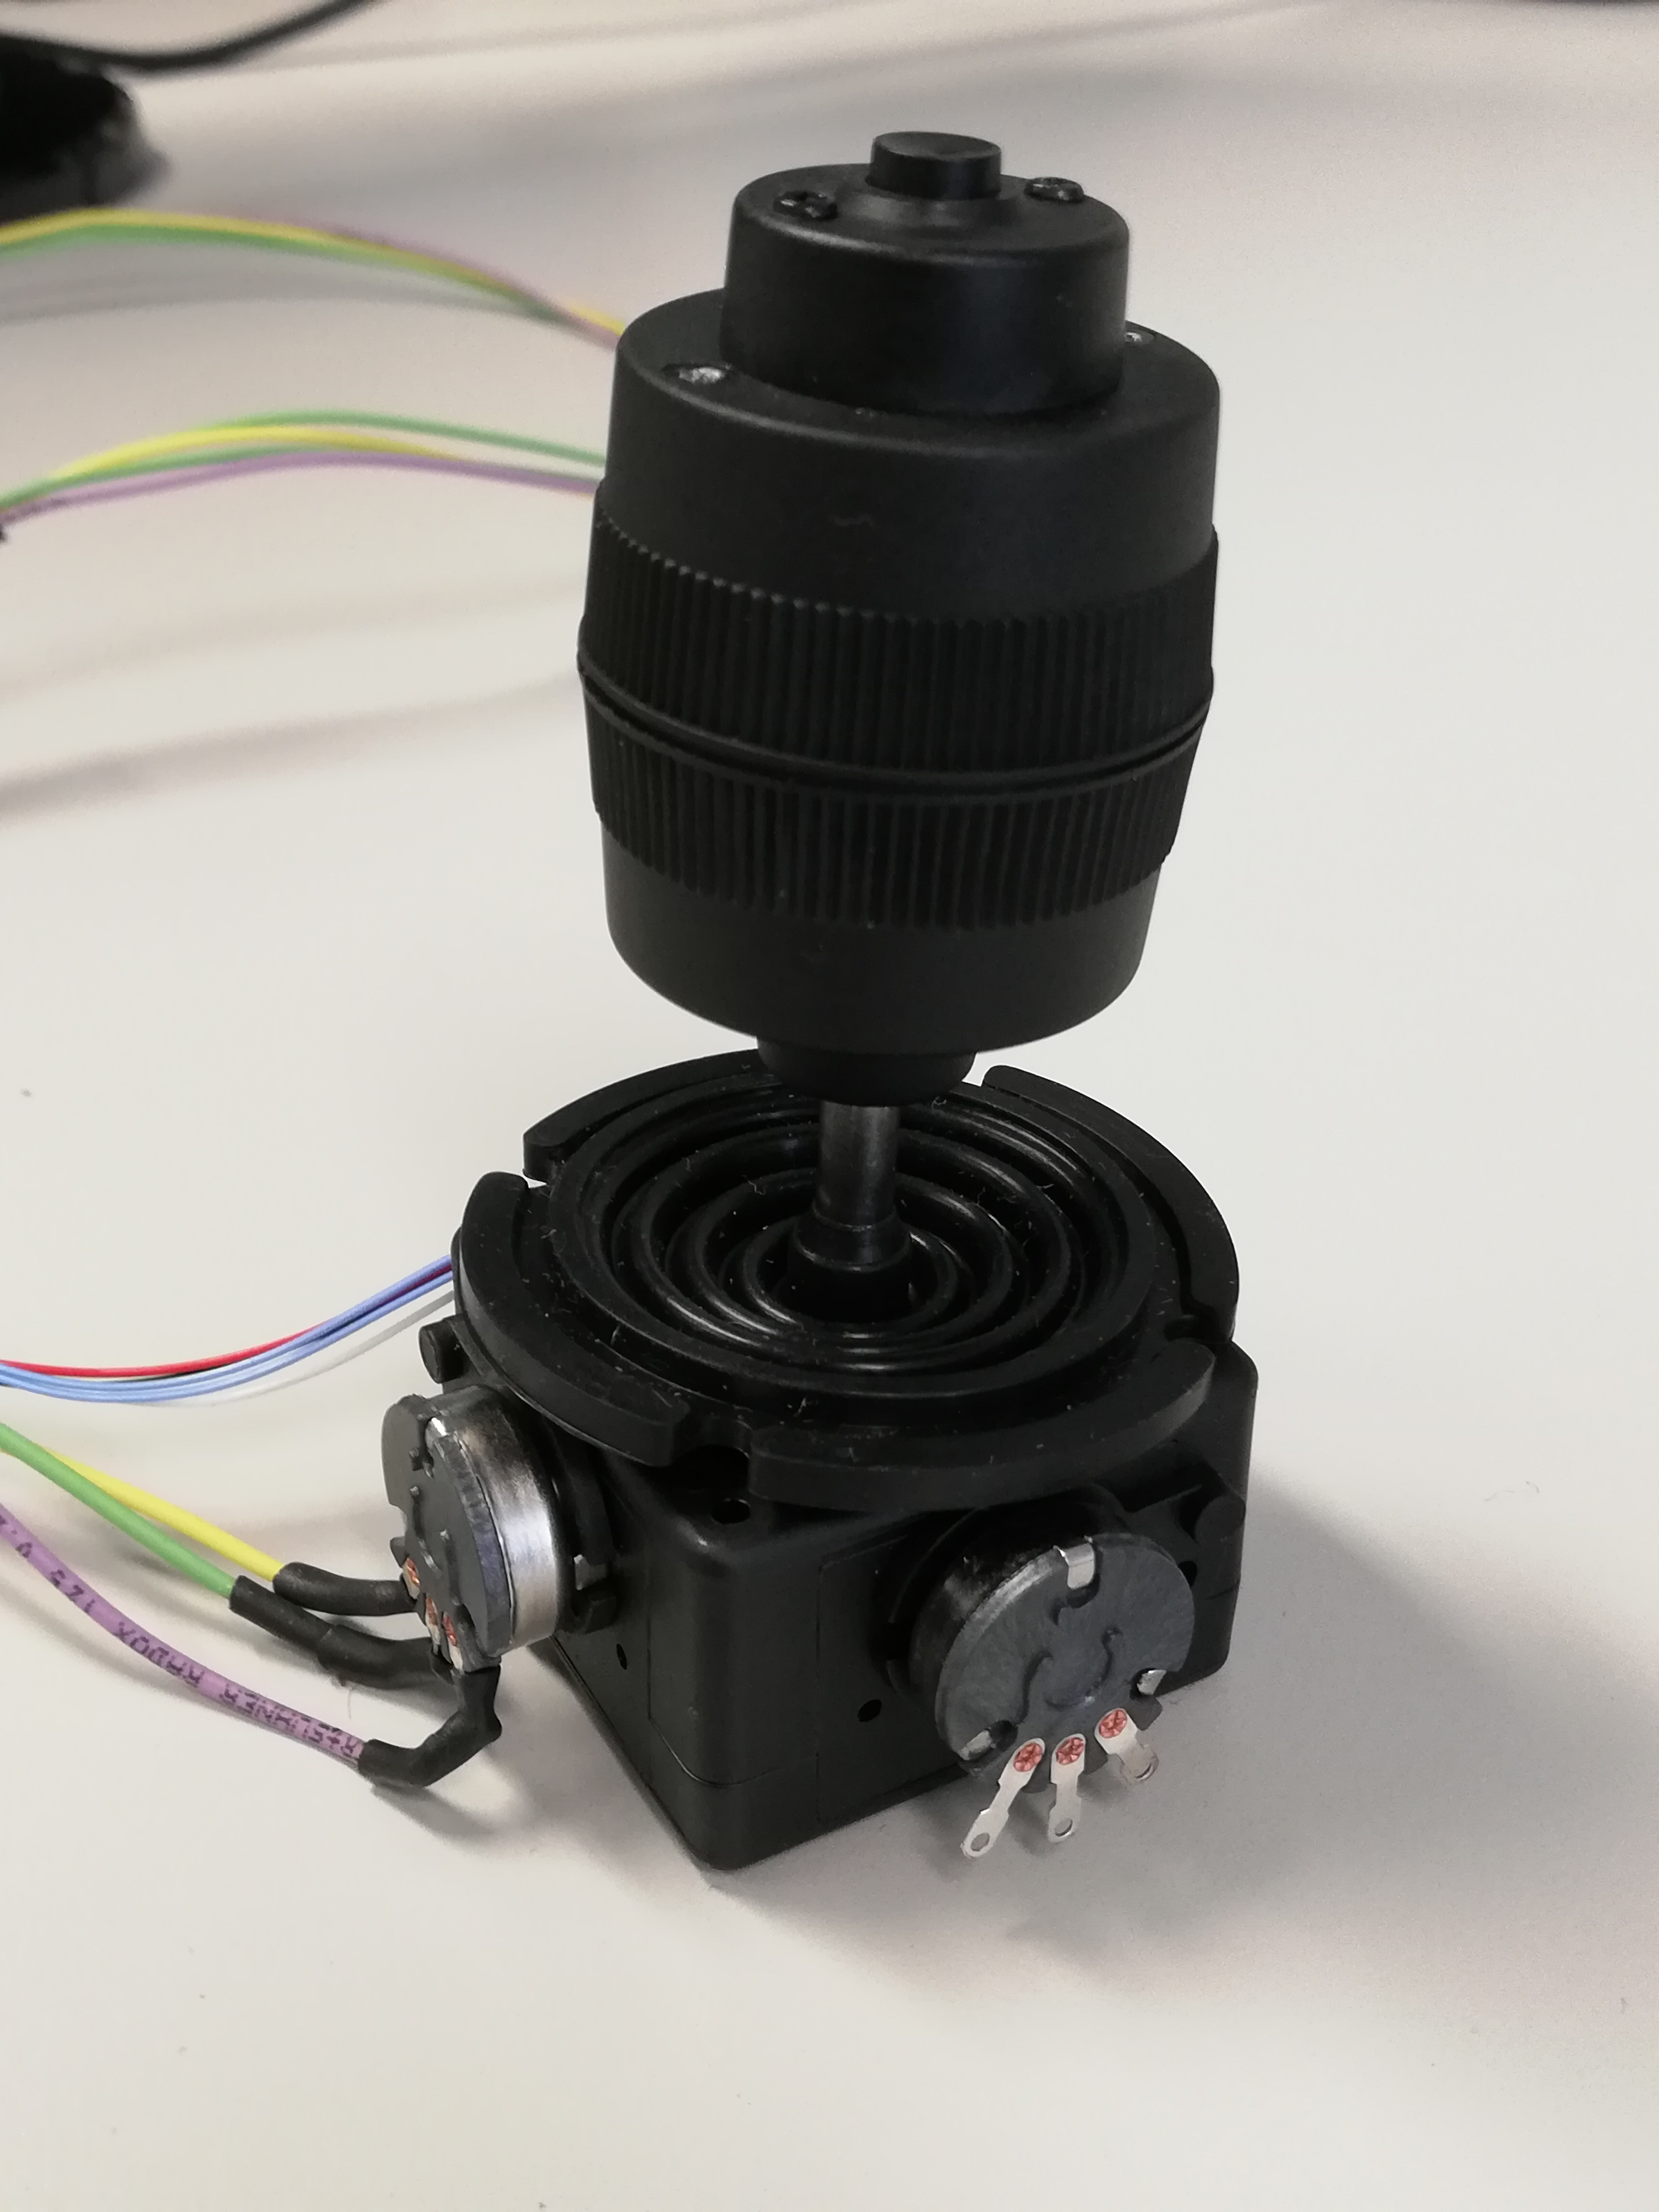
\includegraphics[width=0.6\linewidth]{img/joystick.jpg}
   \caption{Joystick used for the experiments}
   \label{img:joystickimg}
\end{figure}

\section{CatheterLike}\label{sec:catheterlike}
The CatheterLike device is a combination of an analogic sensor and a semi-analogic sensor, figure~\ref{img:catheterimg} and~\ref{img:cathetercad}. The shell of the device was 3D printed in ABS. The device has a handle on the outside that can be pushed and pulled axially coming back automatically to resting position (activated by springs), and can also be rotated over its own axis continuously 360 degrees.\\

The 1st DOF of the catheter is controlled by a 10Kohm and 30mm slide potentiometer. Activated by the push and pull movement on the device, is mapped to the simulated catheter with a Position-velocity mapping.\\

The 2nd DOF is activated by the rotation of the device, mapped Velocity-Velocity to the simulated catheter and controlled by a non-contacting rotatory position sensor, which gives a semi-analogical reading with a 12 BIT resolution per 360 degrees. It Is important to notice that the experiment setup as can be seen in section~\ref{sec:arddevinter} uses an Arduino with a 10BIT ADC channel, which trims the initial sensor's 12BIT resolution.\\

For information about the mapping refer to section~\ref{sec:mapping}.\\

\begin{figure}[ht]
   \centering
   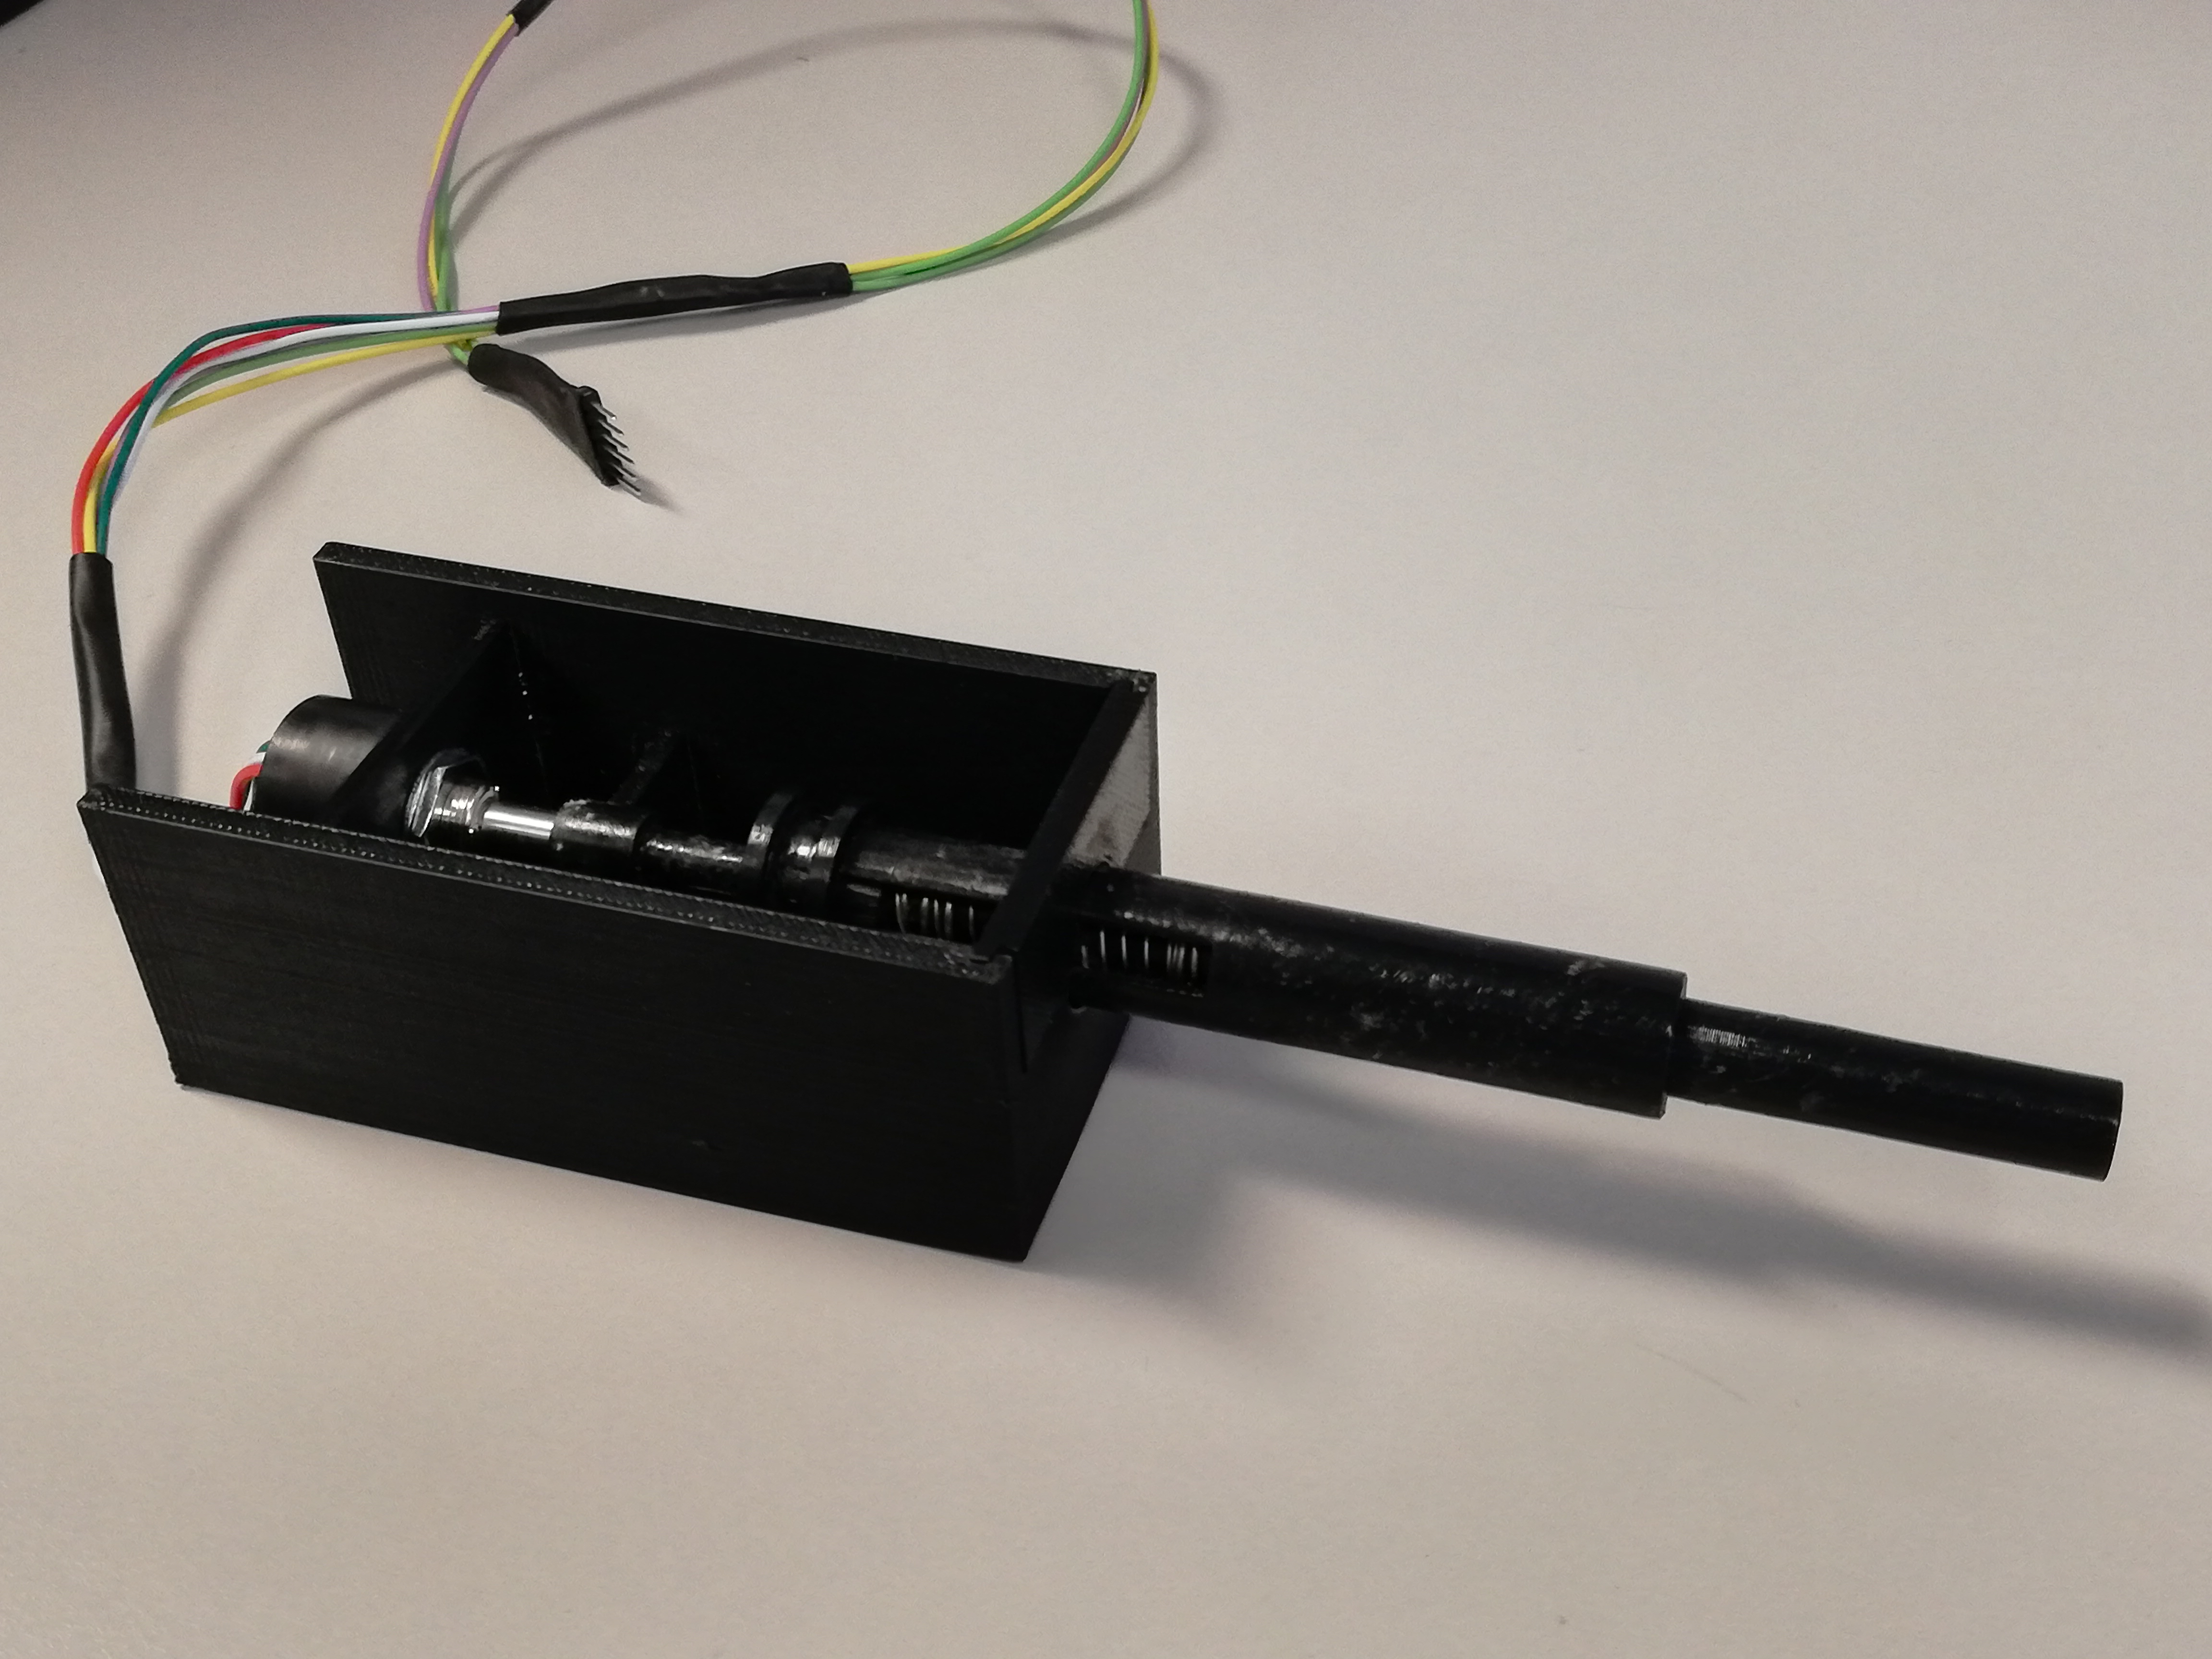
\includegraphics[width=0.7\linewidth]{img/catheter.jpg}
   \caption{Catheter Like device used for the experiment}
   \label{img:catheterimg}
\end{figure}

\begin{figure}[ht]
   \centering
   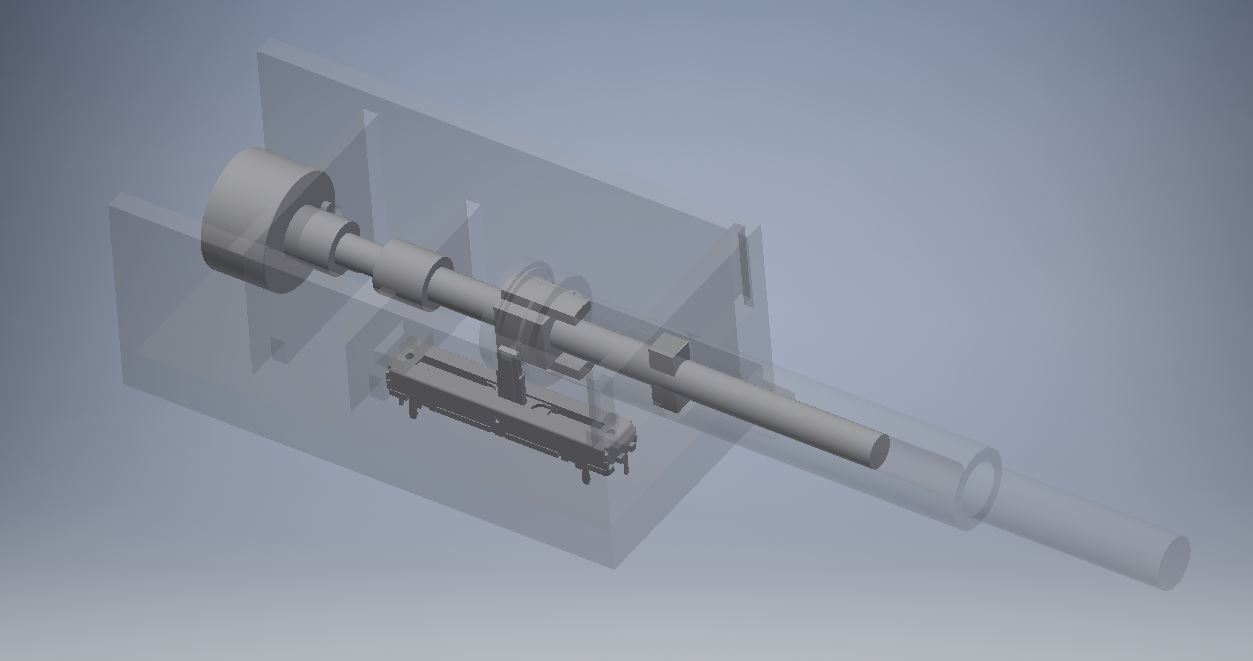
\includegraphics[width=0.7\linewidth]{img/cathetercad.jpg}
   \caption{CAD design of the catheter like design, (Slide Pot PTA3043-2210CIB103) (Rotatory sensor CTS 285CCDFSAAB4C1)}
   \label{img:cathetercad}
\end{figure}

\section{Mapping types, Advantages and Disadvantages}\label{sec:mapping}
Every device with its different type of sensor is better adapted for a specific mapping. This means, how specific movements in each one of the devices, in each one of its degrees of freedom, translates to movements on simulation catheter.\\

The \textbf{PressedTime-Velocity} mapping was created to mitigate the clear disadvantage devices with on-off buttons have against analogical/semi-analogical ones. This disadvantage is due to the fact that on-off devices have always the same speed applied over the catheter. If that speed is too high, it is not possible to apply small movement. On the other hand, if it is too low, it would take too much time to perform long movements. On the contrary, analogical sensor devices have a wide range resolution from where low and high speeds can be applied in the same configuration.\\

This mapping consists in incrementing the output velocity linearly with a defined slope in relation with the time the button was pressed, starting from an initial offset, eq~\ref{eq:1steq}.\\

\begin{equation}
   \scalebox{1.2}{$outputVel=constant+(constant*pressedTime)$}
   \centering
   \label{eq:1steq}
\end{equation}

The \textbf{Position-Velocity} mapping is used in devices with analogical sensors, mapping linearly with a defined slope the position of the sensors to the velocity of the output catheters, eq~\ref{eq:2ndeq}.\\

\begin{equation}
   \scalebox{1.2}{$outputVel=sign(position)*max(0,abs(position-threshold))*constant$}
   \centering
   \label{eq:2ndeq}
\end{equation}

The threshold variable is meant to create a dead zone around the resting point of the device, given that the mechanism that automatically return the device to the resting point is never perfect and it is also important to avoid accidental activation movements on the simulated catheter.\\

The \textbf{Velocity-Velocity} mapping is used for the semi-analogical rotatory sensors, which are able to rotate continuously 360 degrees (multi turn). This method maps the velocity of the device to the velocity of the simulated catheter, multiplied by a constant, eq~\ref{eq:3rdeq}.\\

\begin{equation}
   \scalebox{1.2}{$outputVel=\frac{deviceCount(k)-deviceCount(k-1)}{Ts}*constant$}
   \centering
   \label{eq:3rdeq}
\end{equation}

Using this type of sensors simplify the mechanics of the device but adds an additional challenge when getting the information from the Arduino to Matlab (See Experiment Environment section~\ref{sec:matardinter} for setup). This happens because the sample rate the Arduino board has to sample the device is much faster than the sample rate from Matlab to the Arduino, which makes the simulation to take noisy data and the behavior of the simulation catheter looks highly erratic. In order to overcome this and make the user experience smoother, the Arduino sample rate has to match with Matlab simulation sample rate (Being Ts on eq~\ref{eq:3rdeq} now the Matlab sample rate), making Arduino to implicitly take the average of all the movements between samples.\\

All the advantages and disadvantages are resumed in figure~\ref{img:adtable}.\\

\begin{figure}[ht]
   \centering
   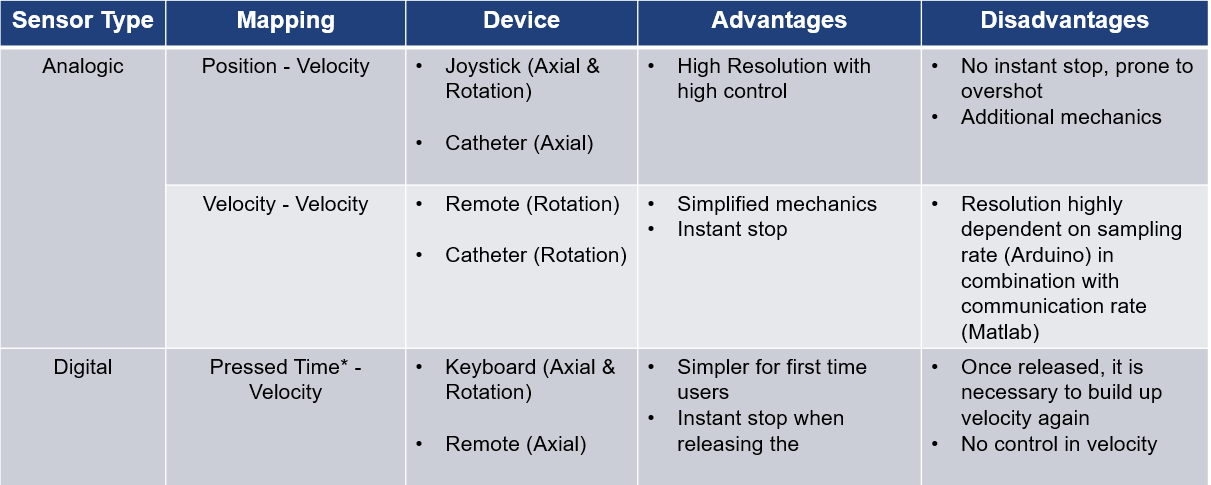
\includegraphics[width=1.0\textwidth]{img/adtable.PNG}
   \caption{Table of advantages and disadvatages of each mapping type}
   \label{img:adtable}
\end{figure}

\cleardoublepage
% !TeX root = /../Report.tex

\chapter{Experiments and Results}\label{sec:experiments}

\section{Experiment Setup}\label{sec:setup}
The hardware of the experiment setup consists of a computer running the Matlab graphic simulation, the four master devices (Keyboard, Remote, Joystick and CatheterLike) and an Arduino board, used to read the sensors of the devices (the keyboard was connected directly to the computer) and communicated with Matlab through USB serial. The diagram is shown in figure~\ref{img:expsetup}.\\

\begin{figure}[ht]
   \centering
   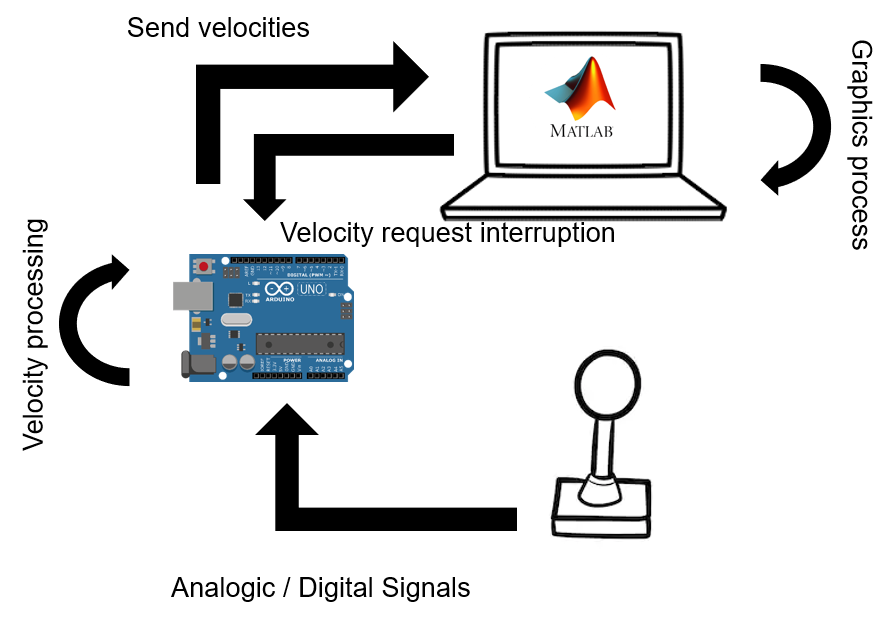
\includegraphics[width=0.7\textwidth]{img/expsetup.PNG}
   \caption{Experiment setup communication diagram}
   \label{img:expsetup}
\end{figure}

\section{Graphic Environment}\label{sec:environment}
The graphic environment is fully developed on Matlab, it consist of a representation of a catheter (With a green square following the tip) in a simulated fluoroscopy image, as surgeons would see it in the operation room, figure~\ref{img:graph}. This means the image showed on screen is a 2D black and withe plain representation. The catheter can be moved in its 2 DOF, being the 1st DOF the axial movement (defined in simulation by the Y coordinate), the catheter would move up and down only. The 2nd DOF is the rotation (defined in simulation as radians starting from the left most possible position of the catheter's tip), which is translated to a left and right movement on the screen.\\

Since the 2nd DOF is defined by the rotation (in radians) of the catheter, some dynamics are implicitly stated in the simulation during the left to right movements. As the image shown is intended to be a 2D representation of an actual 3D catheter in real life, when the catheter is rotating over its own axis a sinusoidal movement can be observed, moving slower when the tip of the catheter is on the most left/right side of the screen and moving fast when the tip is near the center of the catheter.\\

\begin{figure}[ht]
   \centering
   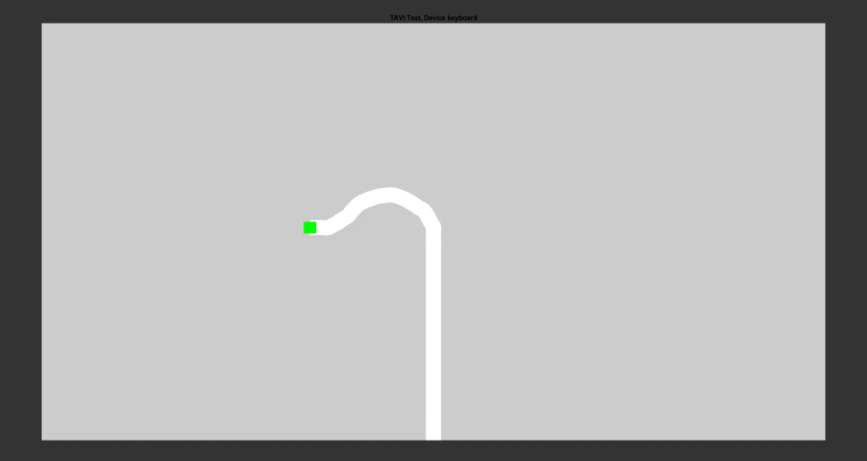
\includegraphics[width=0.7\textwidth]{img/graph.PNG}
   \caption{Default experiment graphic environment}
   \label{img:graph}
\end{figure}

\section{MATLAB/Arduino Interface}\label{sec:matardinter}
The Arduino board and Matlab are connected through USB serial communication. The Arduino board is responsible to sense the devices' sensors. When the Matlab simulation starts, Matlab sends the necessary commands to Arduino in order to set it up for the specific device that is going to be in use, after this the Arduino board starts to capture the states of the sensors instantly.\\

Matlab simulation runs in a loop after setting up all the initial conditions. First it requests the Arduino board for the current states of the device. After it updates the graphics accordingly with the movements reported by Arduino. Lastly it stores the states in a log file, for later data analysis.\\

The Arduino board is programed with serial communication interruptions, which means it is constantly getting the current states of the device and storing them into a buffer. Once the Matlab code request the information, the Arduino board code will be interrupted in order to send the last saved states from the device; once this is done the Arduino board will go back to its state reading task.\\

The only device that works in a different fashion is the keyboard, which is connected directly to the computer through USB. This device interrupts Matlab directly when one of the keys is pressed and stores the device state directly in the simulation environment. In order to avoid adding/subtracting external latency, even though the Keyboard does not interact directly with the Arduino board, the simulation in Matlab runs the communication with the Arduino board, which returns by default the constant from equation~\ref{eq:1steq}. The constant form equation~\ref{eq:1steq} is substituted by the keyboardConsat defined in equation ~\ref{eq:4theq}, with \{-1,0,1\} the possible states of keyboardMatlabState. Then the specific equation for the keyboard changes from~\ref{eq:1steq} to~\ref{eq:5theq}.\\

\begin{equation}
   \scalebox{1.2}{$outputVel=keyboardConst=constant*keyboardMatlabState$}
   \centering
   \label{eq:4theq}
\end{equation}

\begin{equation}
   \scalebox{1.2}{$outputVel=outputVel=keyboardConst+keyboardConst*pressedTime$}
   \centering
   \label{eq:5theq}
\end{equation}


\section{Arduino/Device Interface}\label{sec:arddevinter}
The Arduino board has analogical and digital input in which the devices are directly connected to, according each device sensor types. Once the Arduino board is initialized by Matlab, readings to the corresponding inputs are performed and processed according to the programed mapping type (see section~\ref{sec:mapping}). The processed information is stored in a buffer and the loop keeps running in the same way.\\

\section{Physical Setup}\label{sec:physical}
All the experiments were run in the same environment under the same conditions. An external monitor was setup to run the graphic simulation over a desk with a chair for the experiment candidate to sit. Every device was presented in front the candidate to be taken when necessary according the running experiment, as shown in figure~\ref{img:setupphy}.\\

All the simulations start only once the candidate had performed the first movement. In that moment the simulation starts recording data, and once the simulation time or the goal is reached, it closes itself and immediately launches the next simulation, waiting for the candidate to perform the first movement again, until all the repetitions are finished.\\

\begin{figure}[ht]
   \centering
   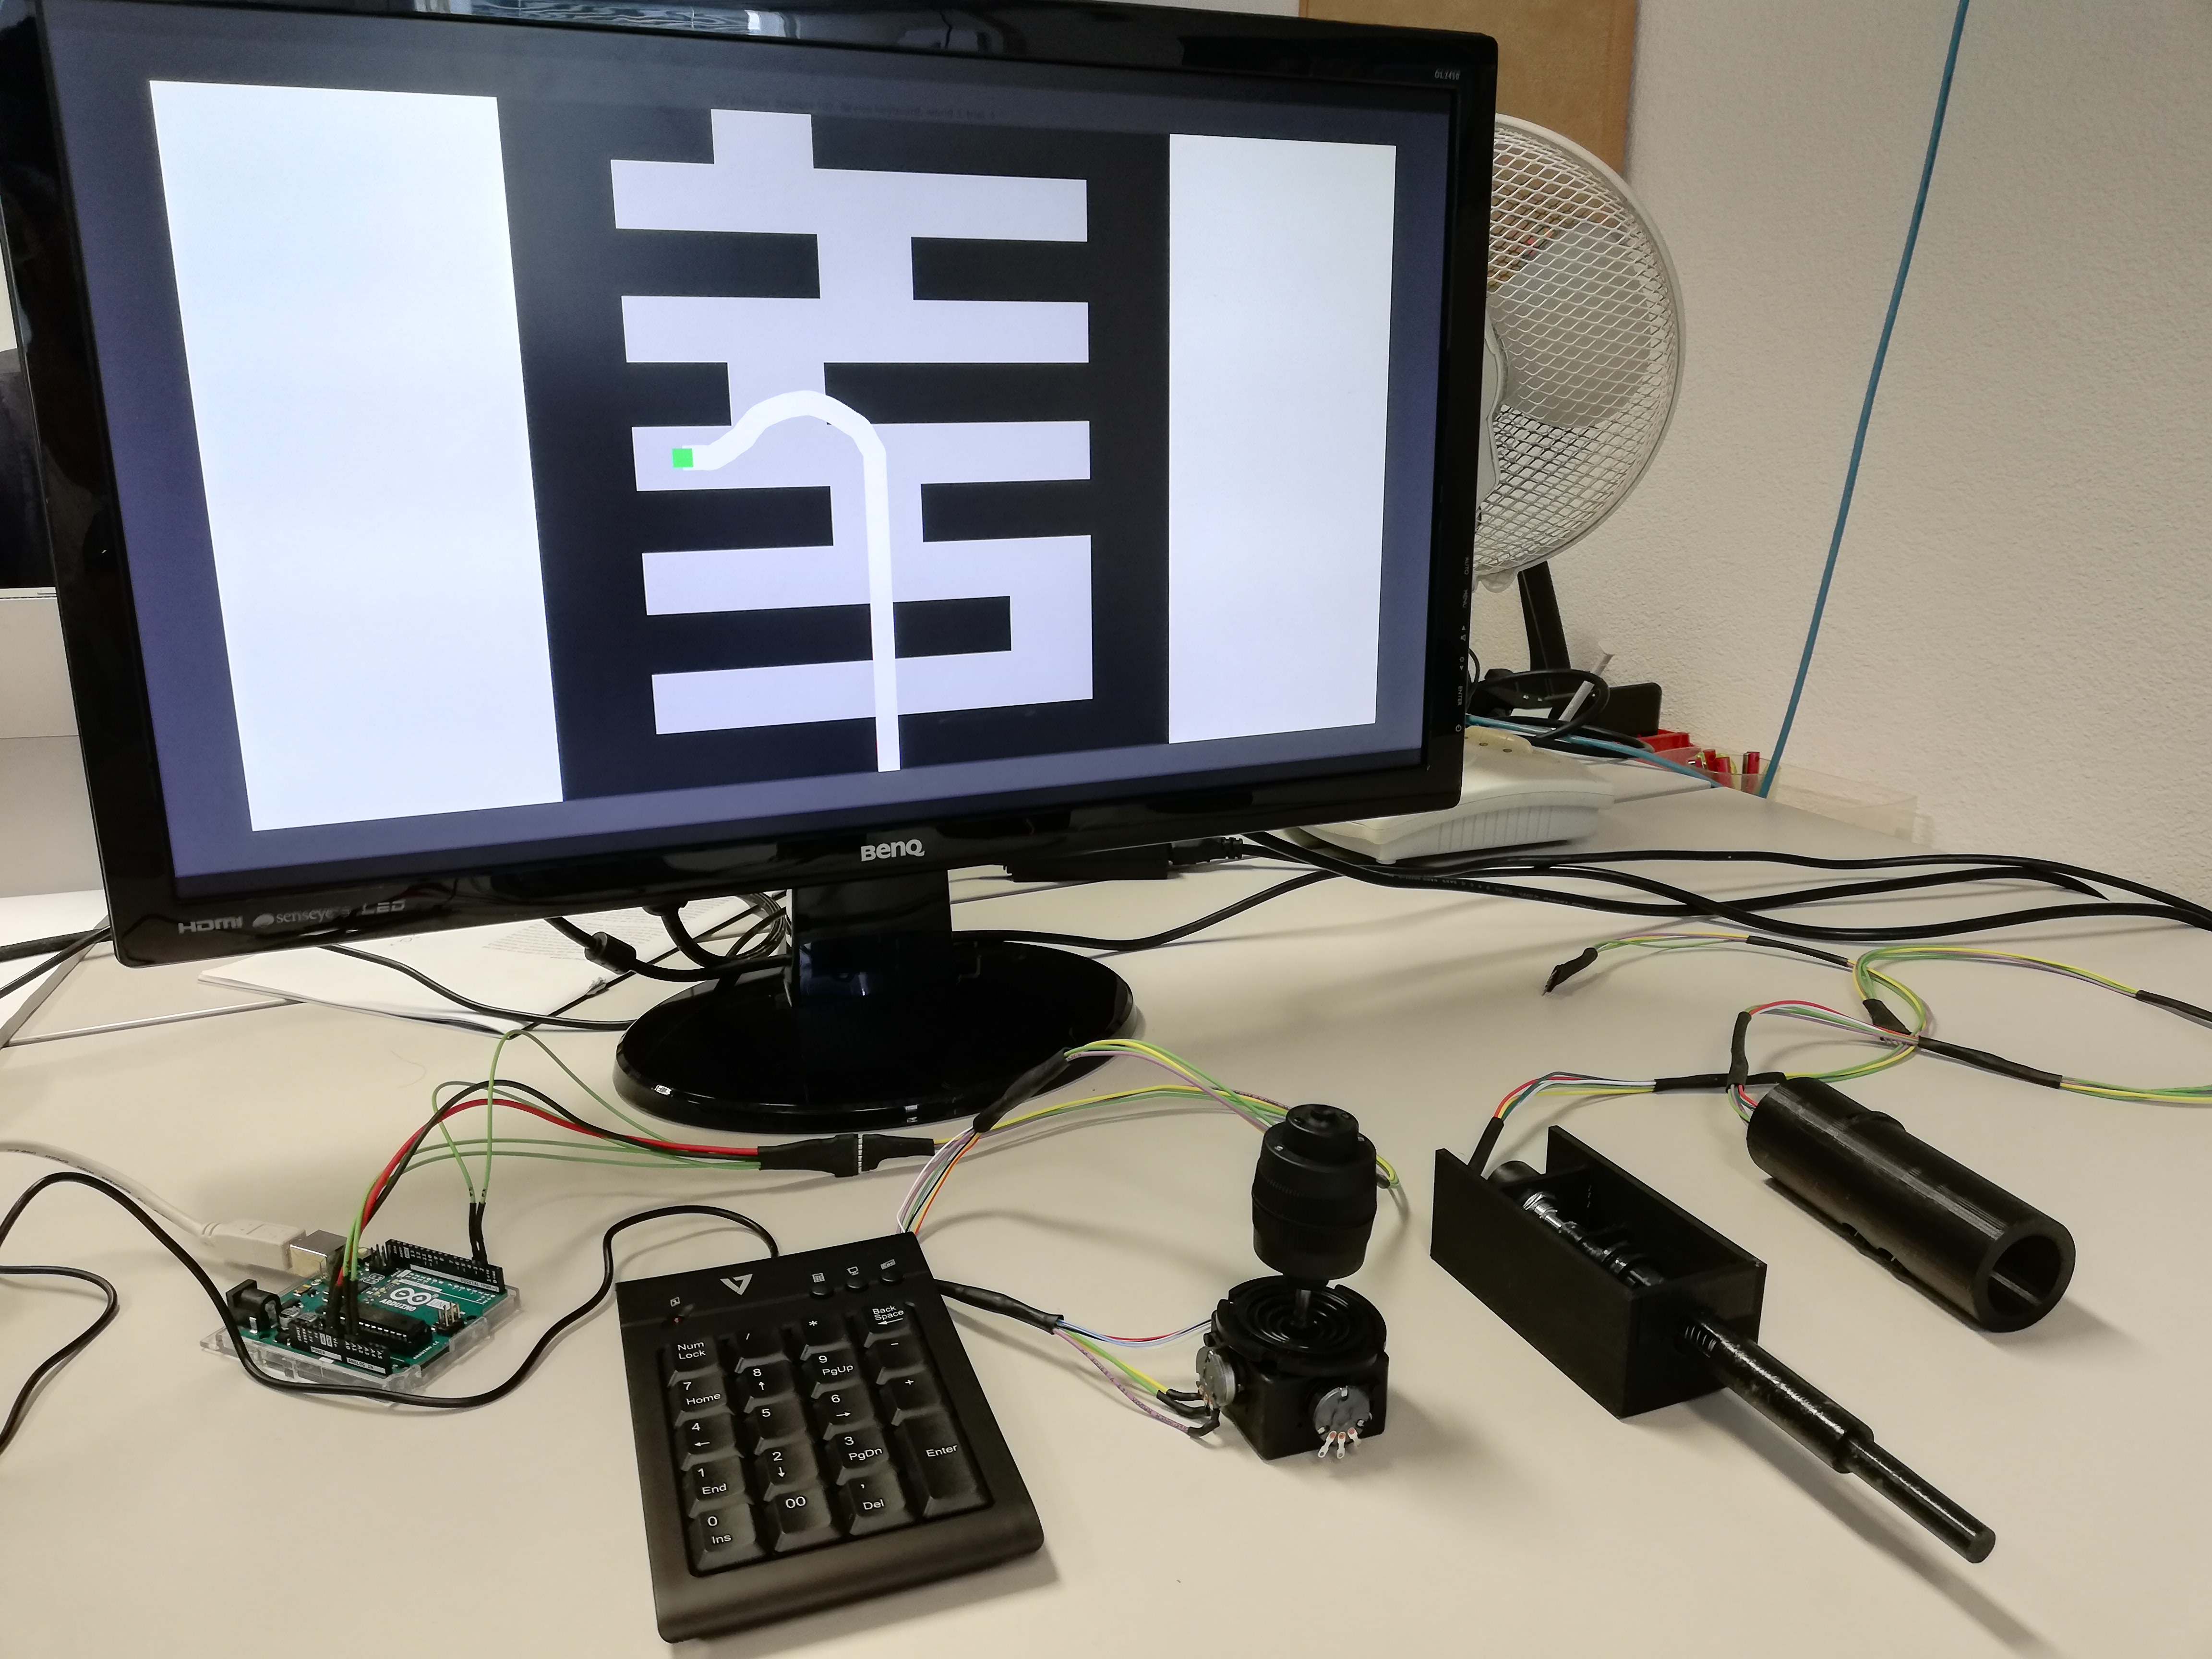
\includegraphics[width=0.7\textwidth]{img/setup.jpg}
   \caption{Physical setup environment used for the experiments}
   \label{img:setupphy}
\end{figure}

\section{Participants Statistics}\label{sec:partstats}
The experiment was conducted by 15 participants, from the 15 participants:
\begin{itemize}
\item  Only 1 of the participants was an expert surgeon in TAVI procedure
 \item The average age of the participants was: 30.23
 \item 46.15 were Male
 \item 	53.85 were Female
\end{itemize}


\section{Instructions}\label{sec:instructions}
Before initiating the experiments, a sheet with the instructions set as the one shown in appendix~\ref{sec:apinst} was handed to each one of the participants.\\


\section{Practice Round}\label{sec:pratround}
Before any experiment was performed, each participant had time to try and play with every device and how it interacts with the graphic simulation on each one of the DOF. An empty world simulation was displayed as shown in figure~\ref{img:graph}. The devices were randomly selected and handed to the participant, who could manipulate the simulated catheter until he/she would decide to stop or 2 minutes maximum had passed.\\


\section{Experiment 1st and 2nd DOF}\label{sec:1stexp}
\subsection{Overview}\label{subsec:1stover}
This experiment was designed to test the performance of the 1st DOF and 2nd DOF of every device independently. The objective is to try to collocate the tip of the catheter (green square) inside a target (red square) that is only moving up and down for the 1st DOF experiment (figure~\ref{img:1stexp}) and left to right for the 2nd DOF experiment (figure~\ref{img:2ndexp}). The target is always initially collocated above the initial tip of the catheter position for the 1st DOF and to the right of the initial tip of the catheter position for the 2nd DOF experiment. The target starts moving automatically once the simulation detects the first movement of the user, following a predefined path for 10 seconds.\\

For each DOF three different predefined paths (worlds) for the target were created, trying to cover two main purposes, the first one was to exploit the capabilities of every device, reaction time, resolution, change of direction, acceleration and deceleration. The second purpose was to simulate movements surgeons would face in a normal TAVI procedure: 1) for the 1st DOF having to pull back rapidly after moving forward and small precise movements when placing the new valve (preventing PVA~\cite{pvl}~\cite{pvl2}) or trying to cross the aortic valve, 2) for the 2nd DOF having to rotate to avoid a blockage in the artery or contacting with the wall of the aortic artery, and small precise rotation movements surgeons need to perform as technique for crossing the aortic valve~\cite{raptech}~\cite{anatomic}.\\

During the 10 seconds of simulation the RMSE between the tip of the catheter and the target is recorded in X and Y coordinates independently. This measurement was selected as it encloses information and gives insight of the experiment purpose previously mentioned.\\

For each one of the DOF every participant had to complete five times each one of the three target's predefined paths, which means 15 randomly ordered repetitions per device. The repetitions were all executed, one device at a time; however, the devices were ordered randomly at the beginning of the experiment. Also, the order on which every DOF experiment was performed, was randomized for every participant.\\

\begin{figure}[ht]
   \centering
   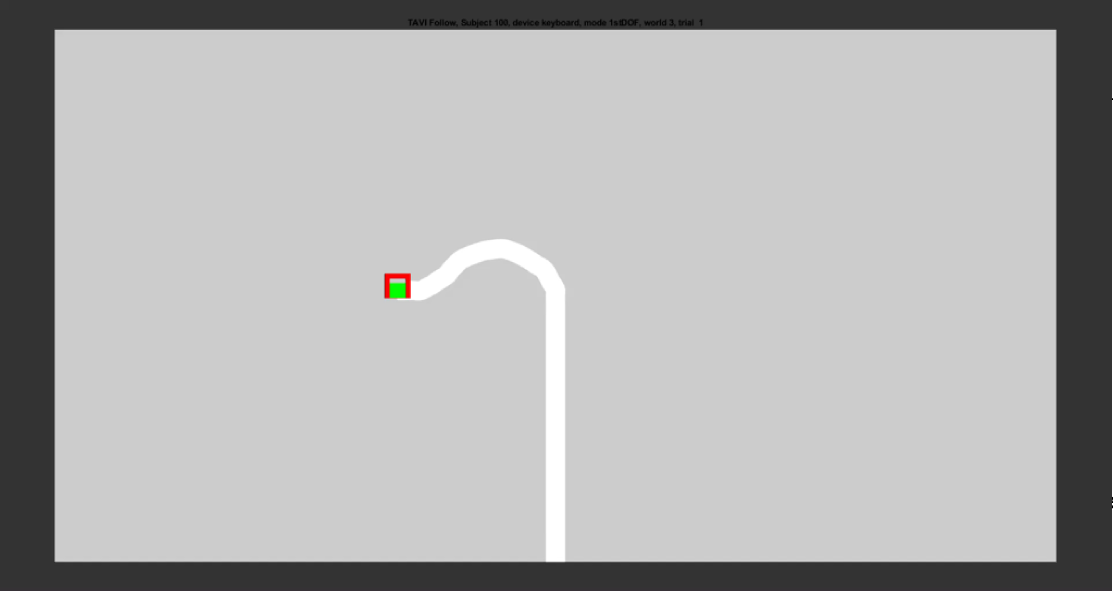
\includegraphics[width=0.8\textwidth]{img/1stexp.PNG}
   \caption{Initial state of the 1st DOF experiment}
   \label{img:1stexp}
\end{figure}

\begin{figure}[ht]
   \centering
   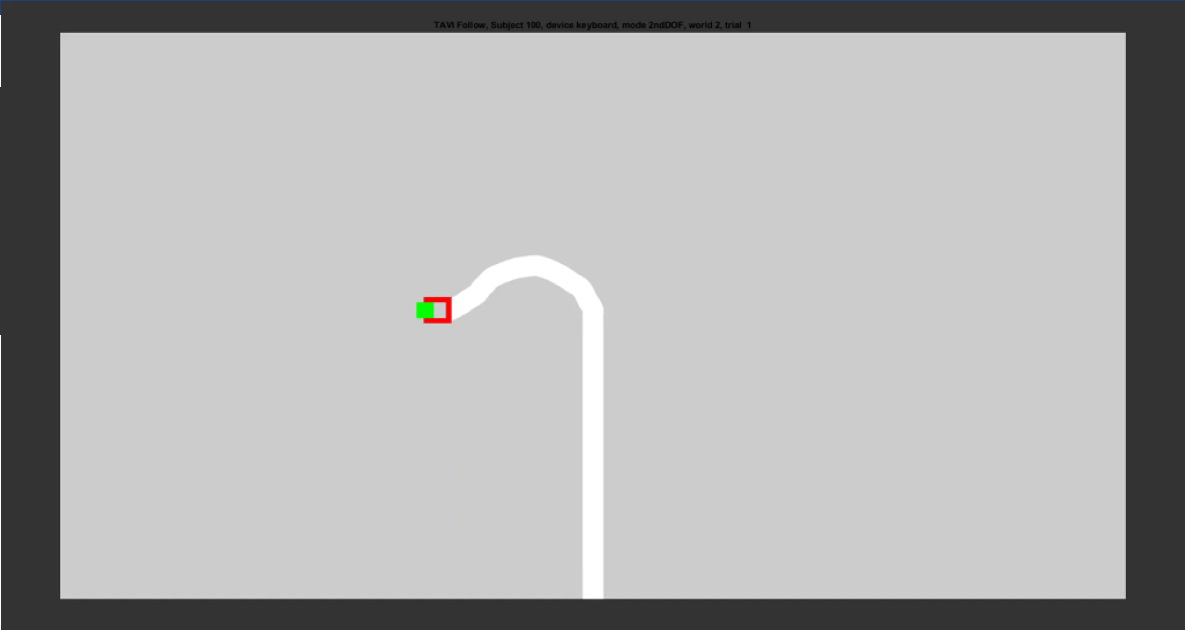
\includegraphics[width=0.8\textwidth]{img/2ndexp.PNG}
   \caption{Initial state of the 2nd DOF experiment}
   \label{img:2ndexp}
\end{figure}

\subsection{Results}\label{subsec:1stres}
All the data from the 15 participants was gathered and the RMSE in both coordinates X and Y for each one of the two DOF computed.\\

As can be observed in figure~\ref{img:1stAvgError}, the 1st DOF experiment shows that the Joystick device has a better performance than the rest of the devices at every different world, followed by the keyboard. However, in figure~\ref{img:1stError} when showing all the samples from the 3 worlds together, two important things are observed. First, the joystick device seems to still show a better performance, but this cannot be concluded when comparing with the keyboard, due to interaction P-Value of 0.006. Secondly, the Joystick device shows a high number of atypical values far away from the box plot, which at first seemed to be failed experiments. However, if those atypical values are traced, the majority of them belong to the first trials of different participants. Thus, if each number of trials is plotted separately as in figure~\ref{img:1stTrainNoExp} (a participant without previous training using Joysticks), a pronounced training curve can be observed. On the other hand, if we plot the same information from a participant that reported experience with the type of the devices used for the experiment as in figure~\ref{img:1stTrainExp}, the superior performance of the Joystick can be observed again followed by the keyboard at every attempt.\\

Another important thing to look at, is the accidental activation error, which means movements in the DOF that was not being tested at each experiment. In order to quantify these involuntary movements, since some of them were too small to be quantified, a percentage of trials where an activation error was present was calculated, as can be observed in figure~\ref{img:1stAct}. It is intuitive that the Keyboard has 0\% of errors due to its digital characteristics, something that would be expected as well from the Remote device, however, that was not the case, since 2.7\% of the cases had an activation error, which can be attributed to experiment errors or issues with the ergonomics of the device. Finally, it can be observed that the catheter had the higher activation error, followed by the joystick.\\

On the 2nd DOF the figure~\ref{img:2ndAvgError} shows that the keyboard had a better performance at every world than any other device, without a clear differentiation between the other three. Also, in the boxplots of figure~\ref{img:2ndError} it can be observed how the Joystick, Remote and Catheter devices have similar distributions, and the keyboard has a better performance with a P-Value of 4.5e-10.\\

The same training behavior as in the 1st DOF experiment can be observed in the 2nd DOF for some of the devices, as shown in figure~\ref{img:2ndTrainNoExp} from a candidate without experience manipulating devices. Also, in figure~\ref{img:2ndAct} the accidental activation error, of the 1st DOF in this case, shows a 0\% in the Keyboard and Remote (devices involving digital inputs in at least one of the two DOF), followed by the Joystick with 3.5\% of test cases and the Catheter with the worst performance with 8\%. Both devices with 0\% proven to be better than the Catheter with P-Value of 0.001, but failed to prove superiority over the Joystick due to an interaction P-Value of 0.03.\\

\begin{figure}[ht]
   \centering
   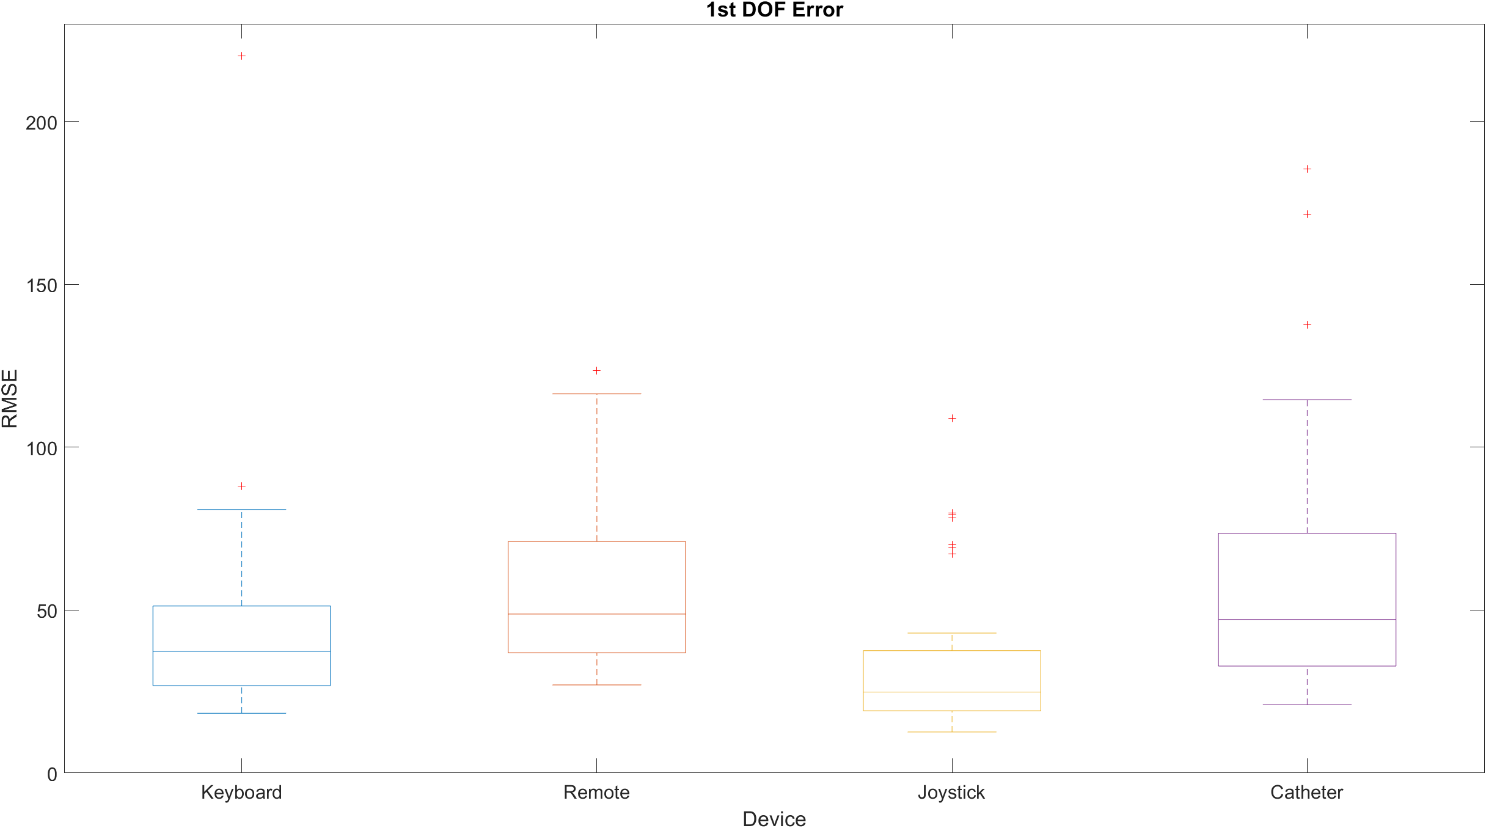
\includegraphics[width=1.0\textwidth]{img/1st/1stError.png}
   \caption{1st DOF RMSE per device across all worlds}
   \label{img:1stError}
\end{figure}

\begin{figure}[ht]
   \centering
   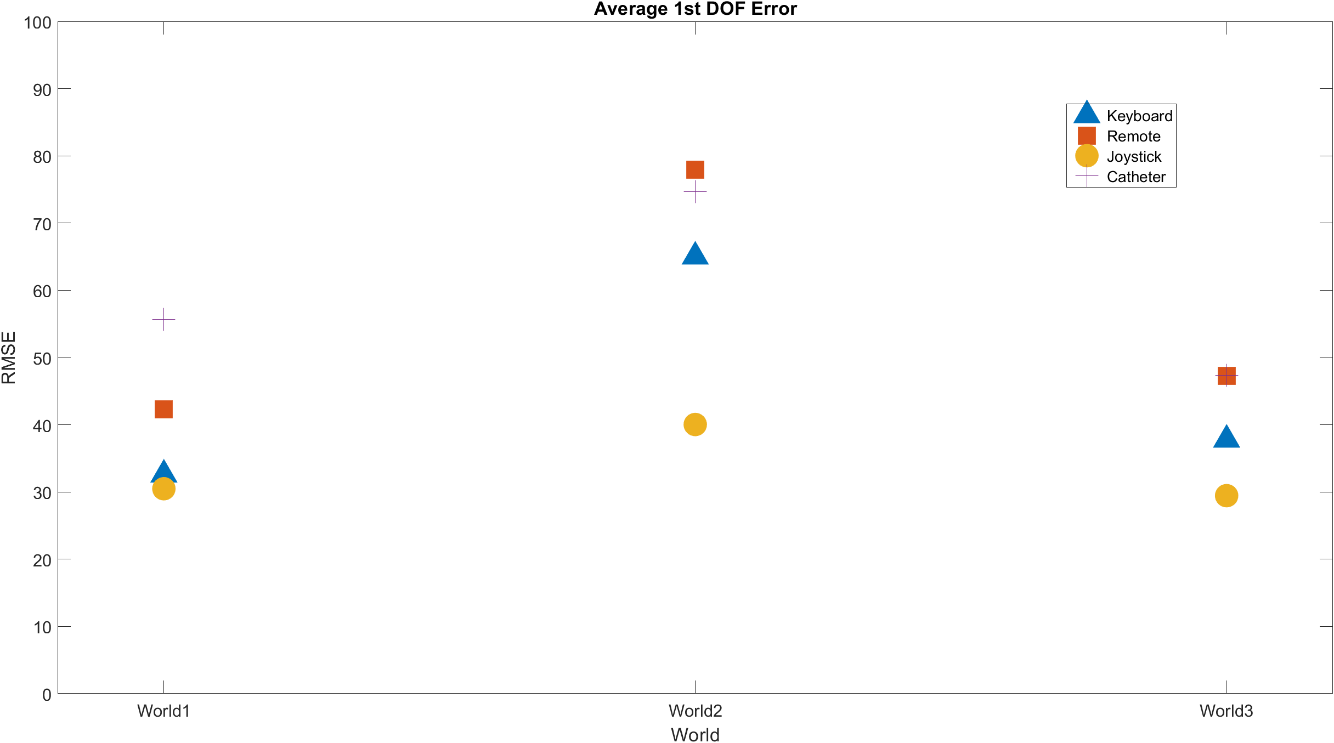
\includegraphics[width=1.0\textwidth]{img/1st/1stAvgError.png}
   \caption{1st DOF RMSE per device at each world}
   \label{img:1stAvgError}
\end{figure}

\begin{figure}[ht]
   \centering
   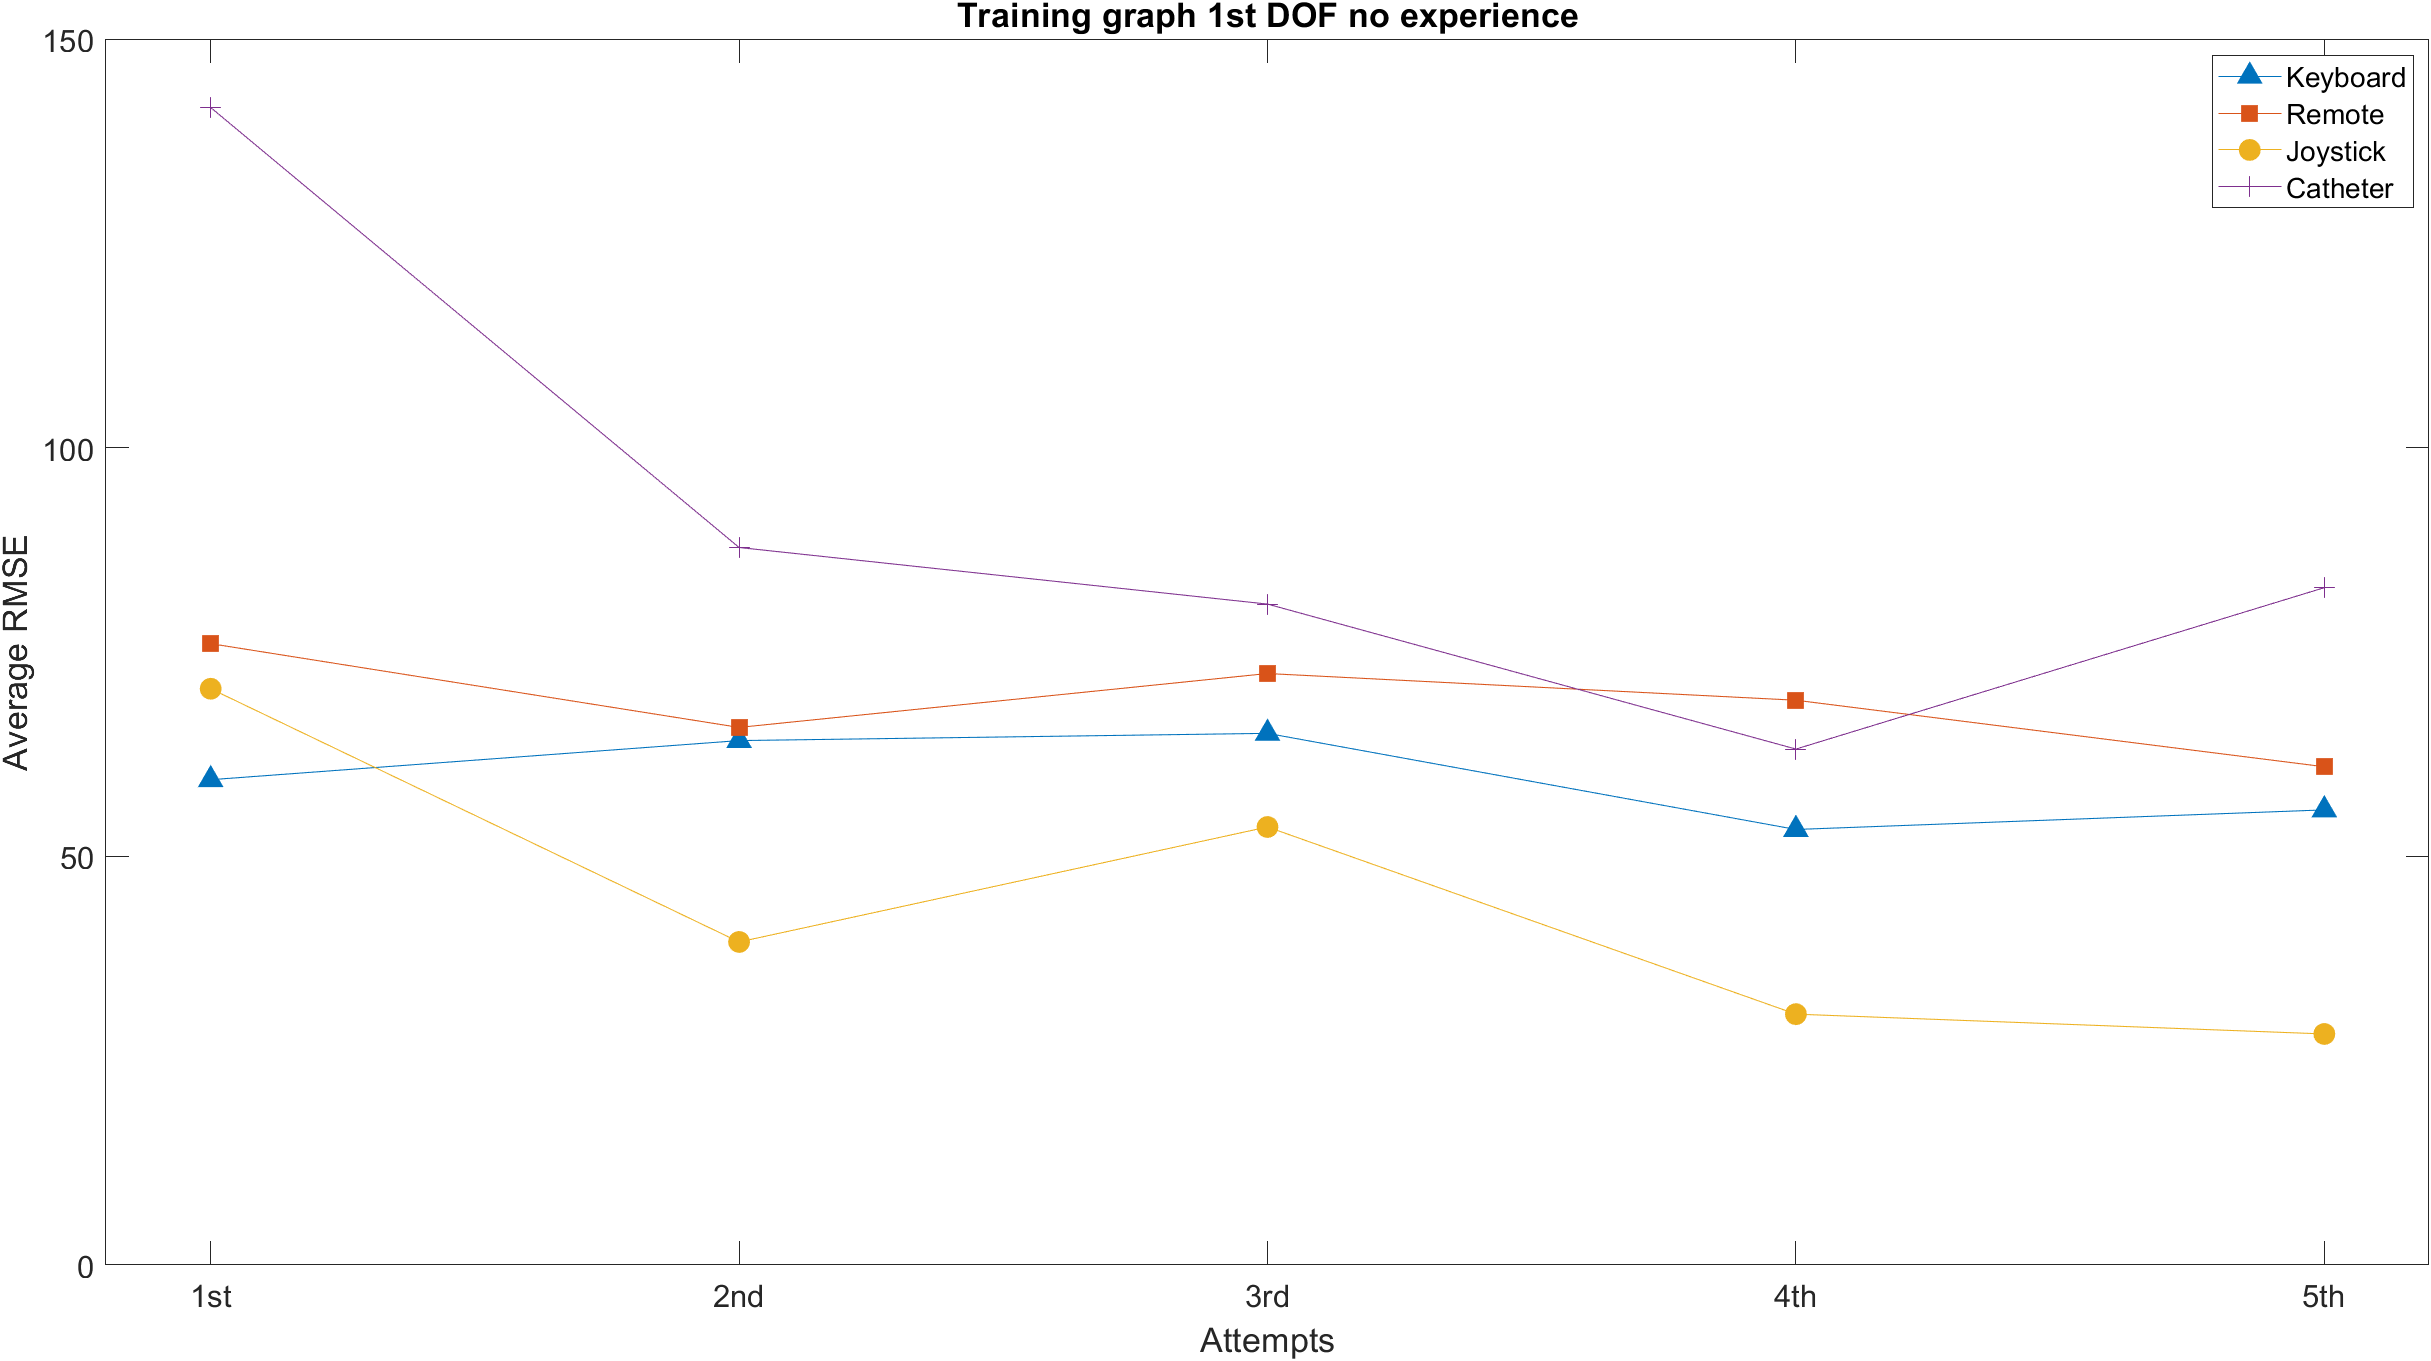
\includegraphics[width=1.0\textwidth]{img/1st/1stTrainNoExp.png}
   \caption{1st DOF RMSE per attempt, participant with no experience}
   \label{img:1stTrainNoExp}
\end{figure}

\begin{figure}[ht]
   \centering
   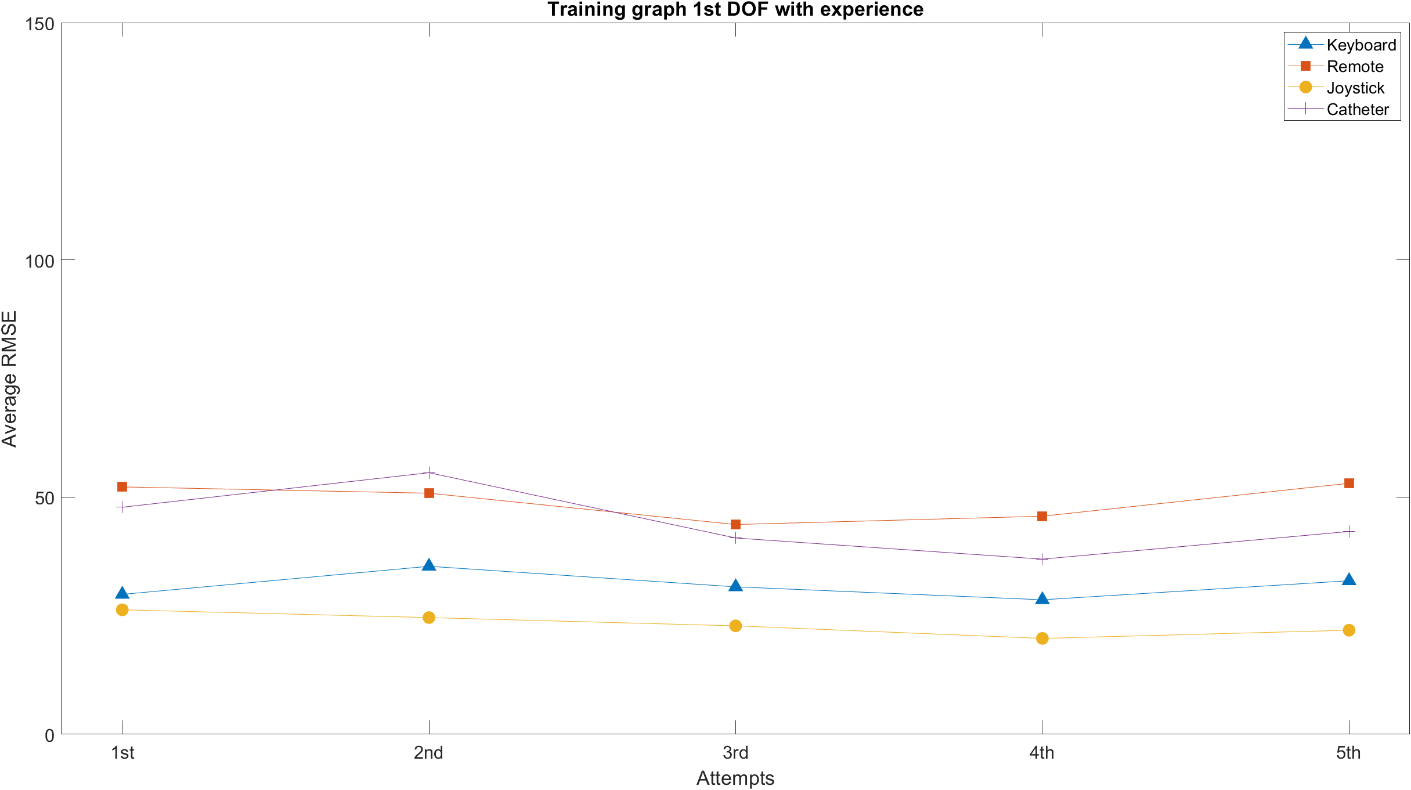
\includegraphics[width=1.0\textwidth]{img/1st/1stTrainExp.png}
   \caption{1st DOF RMSE per attempt, participant with experience}
   \label{img:1stTrainExp}
\end{figure}

\begin{figure}[ht]
   \centering
   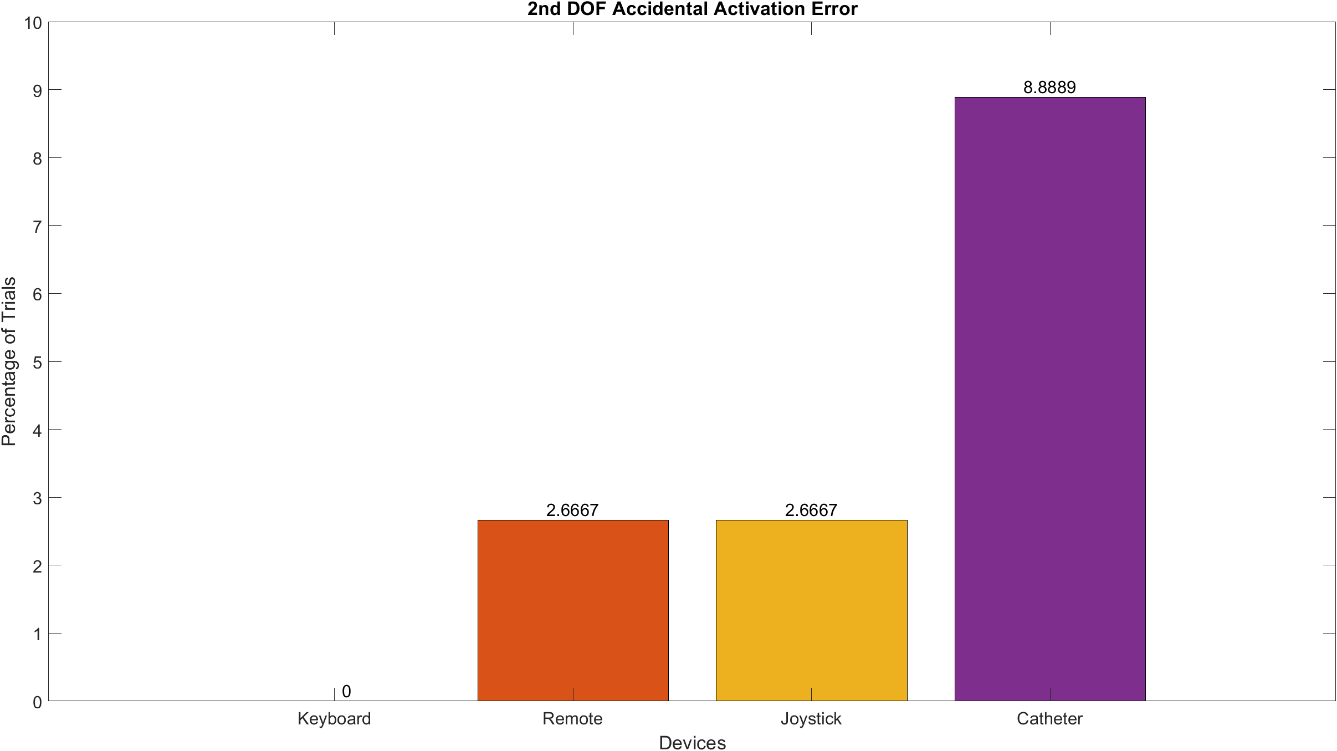
\includegraphics[width=1.0\textwidth]{img/1st/1stAct.png}
   \caption{2nd DOF Activation error while performing 1st DOF experiment}
   \label{img:1stAct}
\end{figure}

\begin{figure}[ht]
   \centering
   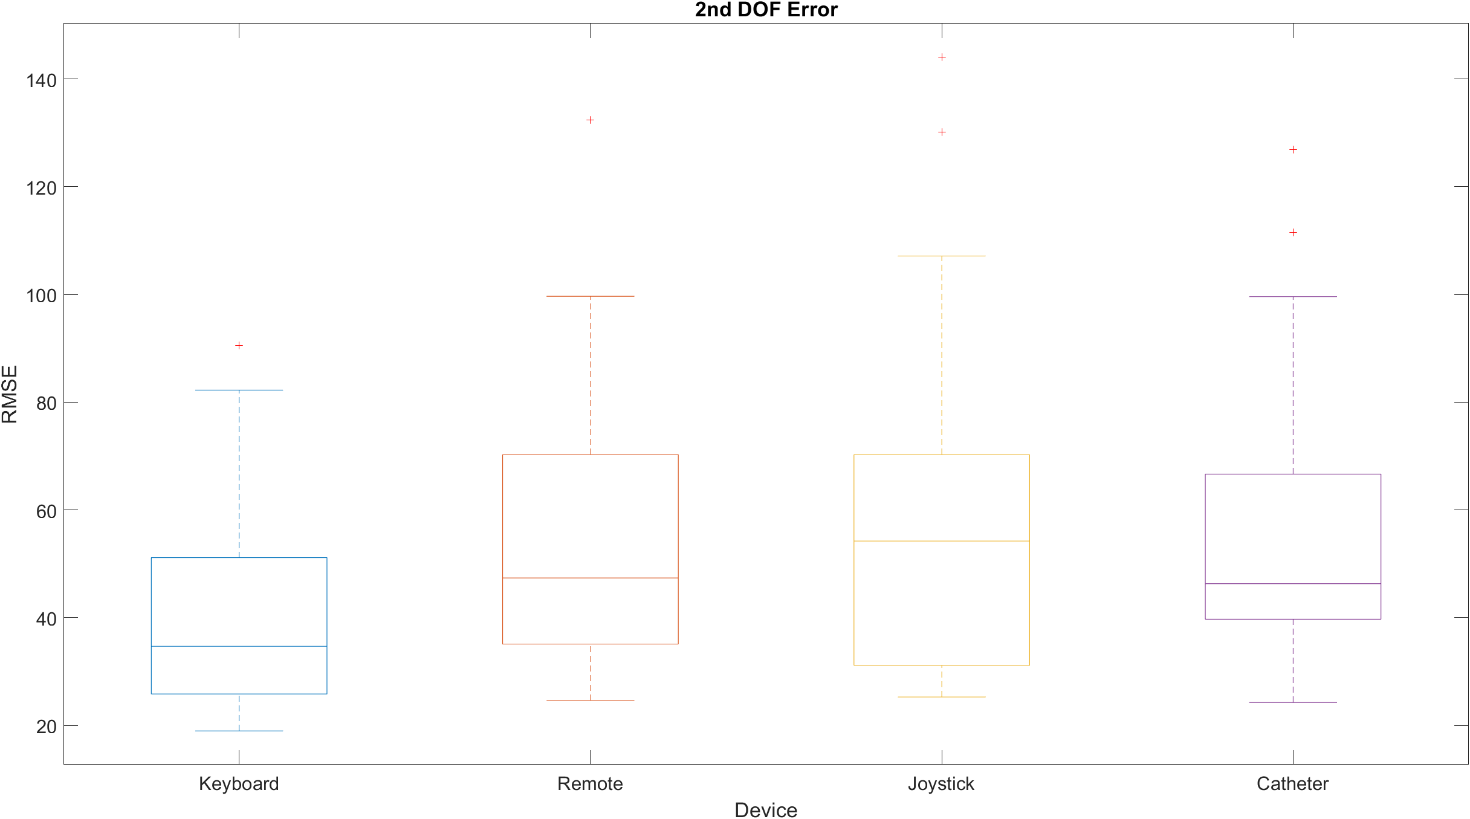
\includegraphics[width=1.0\textwidth]{img/2nd/2ndError.png}
   \caption{2nd DOF RMSE per device across all worlds}
   \label{img:2ndError}
\end{figure}

\begin{figure}[ht]
   \centering
   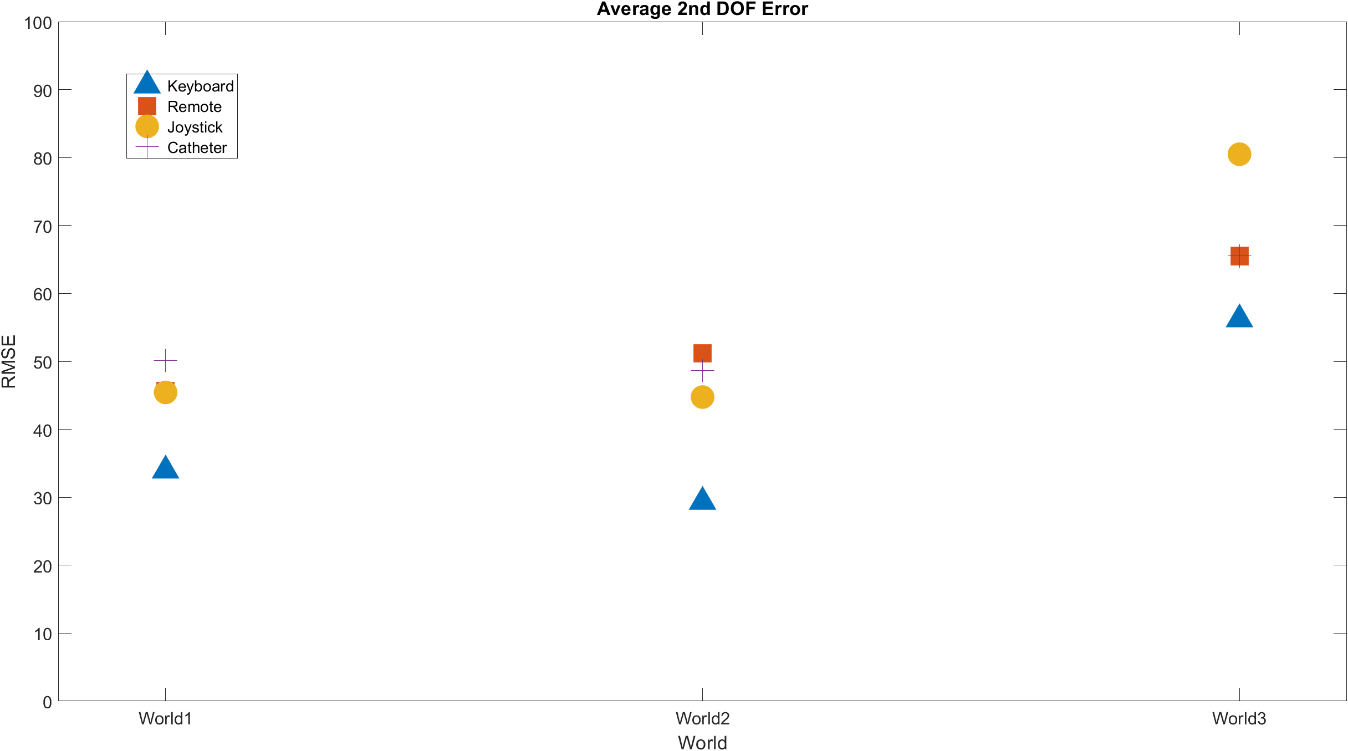
\includegraphics[width=1.0\textwidth]{img/2nd/2ndAvgError.png}
   \caption{2nd DOF RMSE per device at each world}
   \label{img:2ndAvgError}
\end{figure}

\begin{figure}[ht]
   \centering
   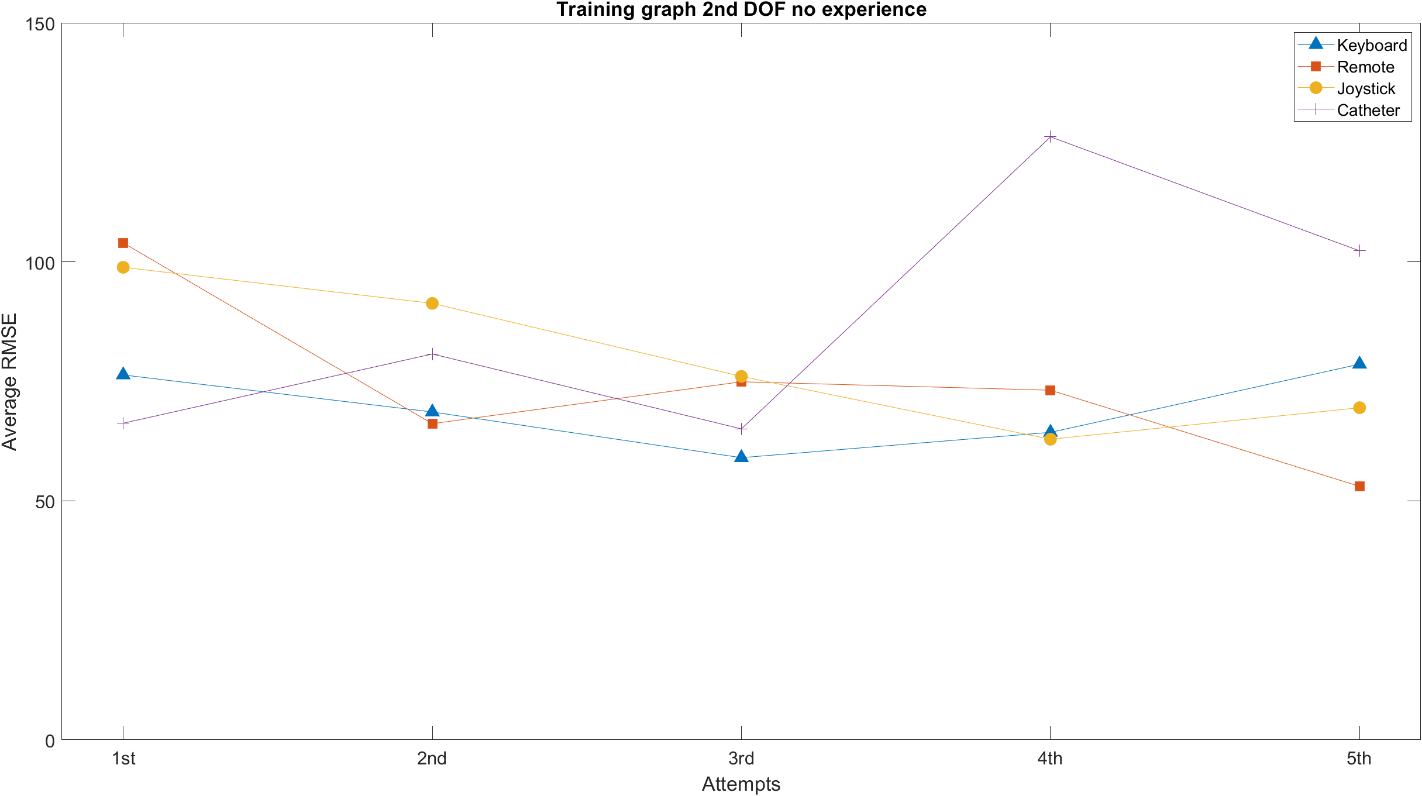
\includegraphics[width=1.0\textwidth]{img/2nd/2ndTrainNoExp.png}
   \caption{2nd DOF RMSE per attempt, participant with no experience}
   \label{img:2ndTrainNoExp}
\end{figure}

\begin{figure}[ht]
   \centering
   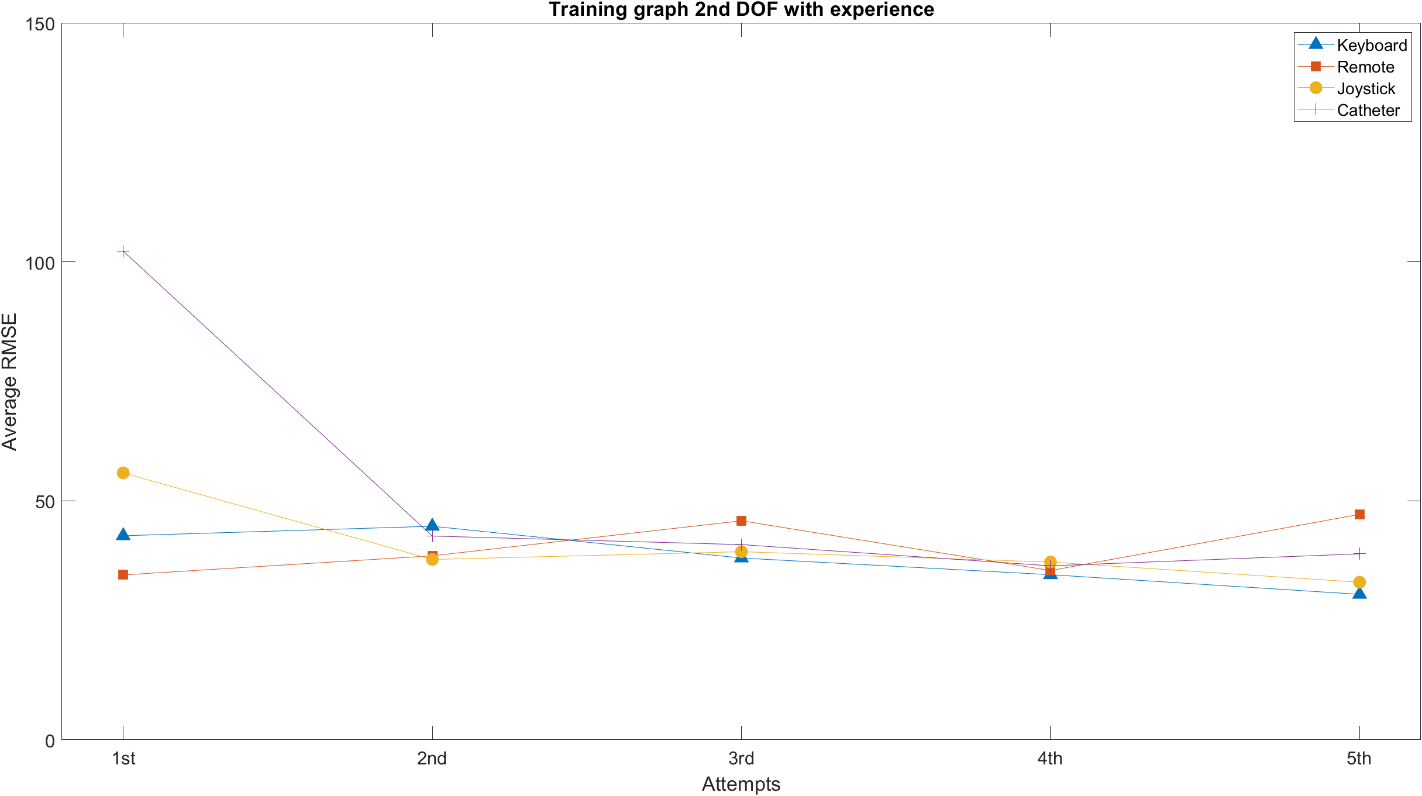
\includegraphics[width=1.0\textwidth]{img/2nd/2ndTrainExp.png}
   \caption{2nd DOF RMSE per attempt, participant with experience}
   \label{img:2ndTrainExp}
\end{figure}

\begin{figure}[ht]
   \centering
   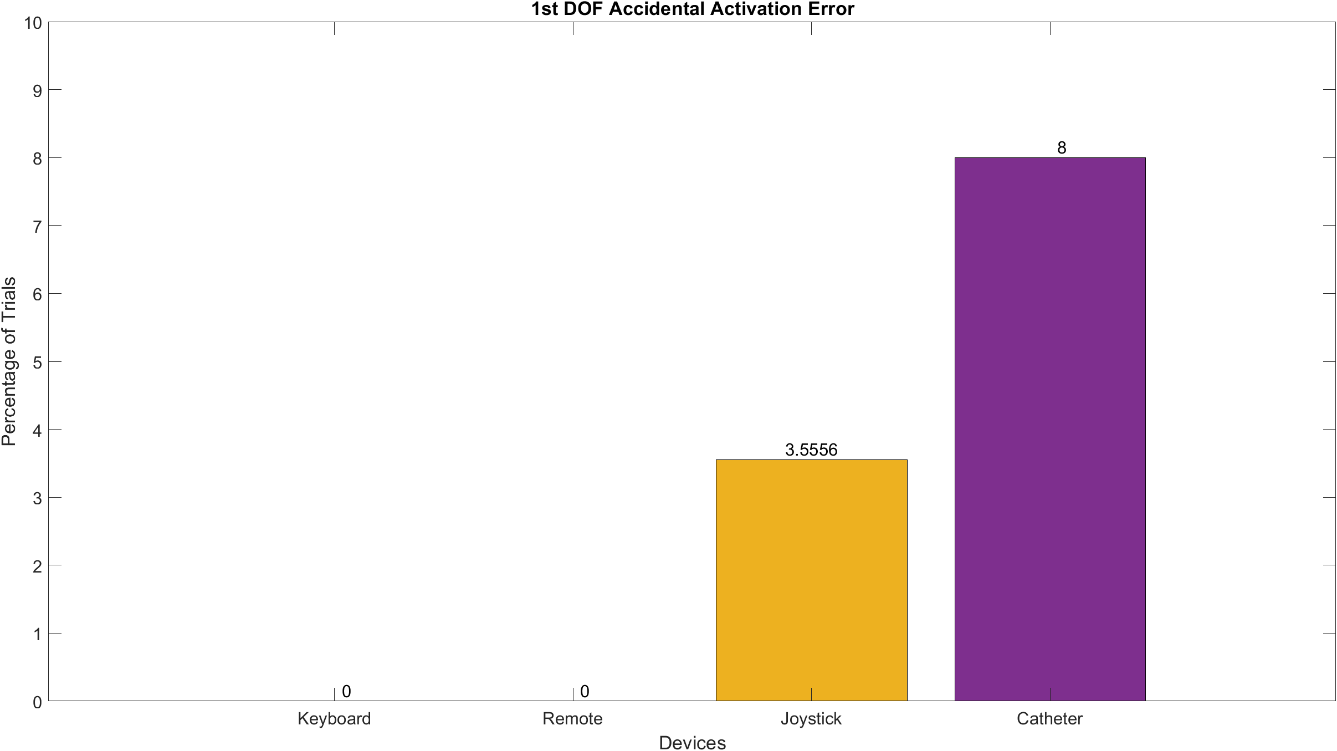
\includegraphics[width=1.0\textwidth]{img/2nd/2ndAct.png}
   \caption{1st DOF Activation error while performing 2nd DOF experiment}
   \label{img:2ndAct}
\end{figure}
\clearpage

\section{Experiment Maze}\label{sec:expmaze}
\subsection{Overview}\label{subsec:2ndover}
This experiment was designed to test the joint performance of the two DOF of every device. The objective is to navigate the tip of the simulated catheter (green square) through a one-way maze as shown in figure~\ref{img:maze}, until reaching the top part of the maze. The users were instructed (as shown in appendix~\ref{sec:apinst}) to navigate the maze keeping the maximum distance to the walls as possible, avoiding collisions and reaching the top wall of the maze in the minor time possible.\\

The simulation starts recording the data when the first movement of the user is detected. In case of collision with a wall, the tip of the catheter stops moving and changes color from green to red (as shown in figure~\ref{img:mazeColl}), indicating a collisions status. In order to clear the collision the user has to back off, any other movement that would keep the collision is not permitted and would not move the simulated catheter at all. Once the tip of the simulated catheter touches the upper wall (as shown in figure~\ref{img:mazeEnd}) the simulation stops.\\

In order to exploit all the capabilities of each device, two different mazes (worlds) were used for this experiment. The first maze (world1) has longer stretches in the 1st DOF, occasionally stopped by a short rotation movement, in order to simulate the first fast strokes the surgeons have to perform in order to reach the aortic arch, if a blockage is found, a small rotation is made and then the surgeon keeps moving forward. The second one (world2) with higher alternation between left/right and up/down movements, simulating scenarios where surgeons have to maneuver both DOF at the same time, such as when they cross the aortic valve~\cite{raptech}~\cite{anatomic}.\\

For this experiment three main metrics were measured, Time to complete the experiment, Number of collisions and Dimensionless squared Jerk. These metrics were selected since they enclose relevant information on the capabilities of the devices and how suitable to perform the tasks they are. Time to complete the tasks is of high importance, since one of the objectives of a Teleoperated robots is to reduce the radiation exposure both, to patients and practitioners. Number of collisions is important to give an insight of the maneuverability of every device (acceleration rate, deceleration rate, precision, among others) which is highly important for patient safety. The dimensionless squared jerk has been previously used in similar studies to asses performance of catheter trajectories~\cite{dsj}~\cite{dsj2}, it is useful to describe the smoothness of the path as well as the accelerations and decelerations, while being independent of time and longitude of the path. The formula to calculate this is described in equation~\ref{eq:dsjeq} where TP is the experiment time (from ti to te) and PL the path length of the trajectory followed by the user.\\

\begin{equation}
   \scalebox{1.5}{$Jd=(\int_{ti}^{te}(\dddot{x}(t))^2 + (\dddot{y}(t))^2 dt)*\frac{Tp^5}{PL^2}$}
   \centering
   \label{eq:dsjeq}
\end{equation}

For each one of the mazes every participant had to complete 5 repetitions, which means 10 randomly ordered repetitions per device. The repetitions were executed, one device at a time; however, the devices were ordered randomly at the beginning of the experiment.\\

\begin{figure}[ht]
   \centering
   
\includegraphics[width=1.0\textwidth]{img/maze/maze.png}
   \caption{Initial state of the experiment maze}
   \label{img:maze}
\end{figure}

\begin{figure}[ht]
   \centering
   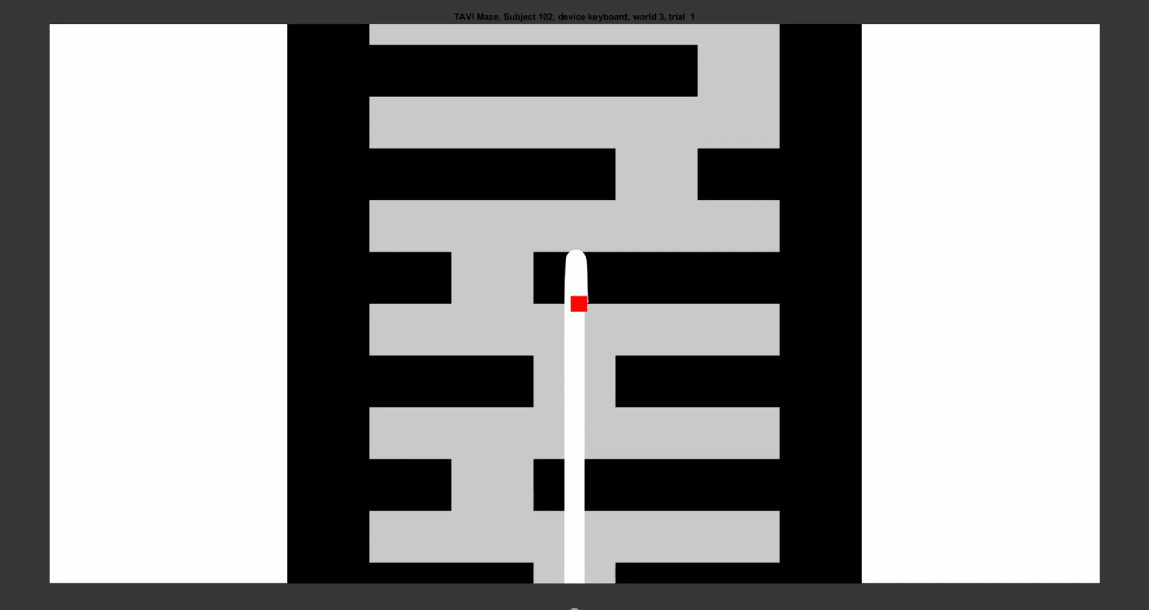
\includegraphics[width=1.0\textwidth]{img/maze/mazeColl.png}
   \caption{Collision during maze experiment}
   \label{img:mazeColl}
\end{figure}

\begin{figure}[ht]
   \centering
   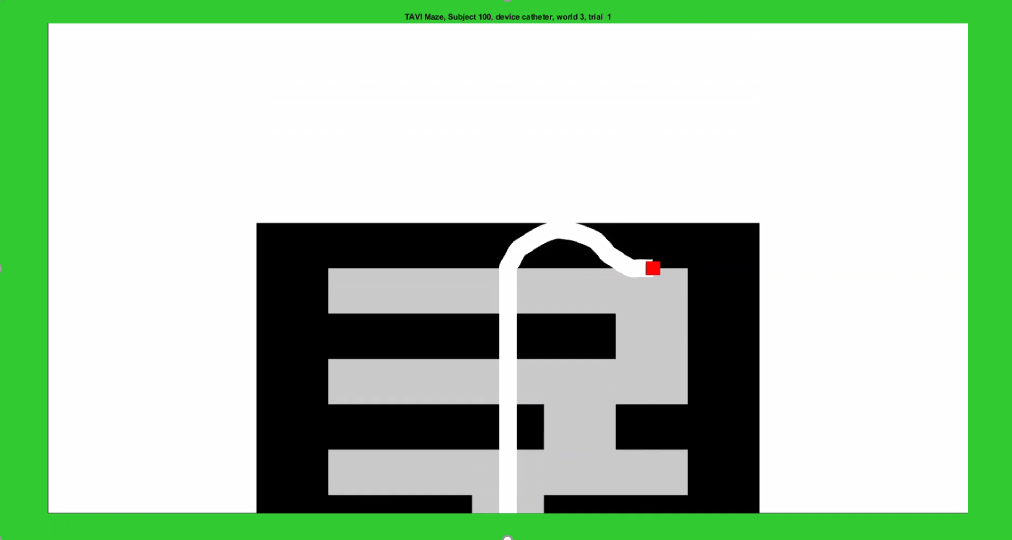
\includegraphics[width=1.0\textwidth]{img/maze/mazeEnd.png}
   \caption{End of maze experiment when colliding with upper wall}
   \label{img:mazeEnd}
\end{figure}

\subsection{Results}\label{subsec:2ndres}
The Time result of the experiment were not statistically conclusive, since interaction with P-Value $<$ 0.05 was always present in the comparison between all the devices. As can be seen in figure~\ref{img:mazeAvgTime}, the Keyboard and the Joystick had a close average time in world1, however, in world2 (with the long stretches) Keyboard dominates. This can be related to the easy control of the keyboard without any training given the immediate stop advantage, as mentioned in figure~\ref{img:adtable}, this allows the user to advance confidently with high velocity and without expecting a collision. Overall it can be observed in figure~\ref{img:mazeTime} that the lowest times were achieved with the Keyboard and Joystick; however, the distribution in the upper quartile in the joystick device as with the remote is widely spread, which as in the experiment for the 1st DOF and 2nd DOF may be attributed to the learning curve.\\

\begin{figure}[ht]
   \centering
   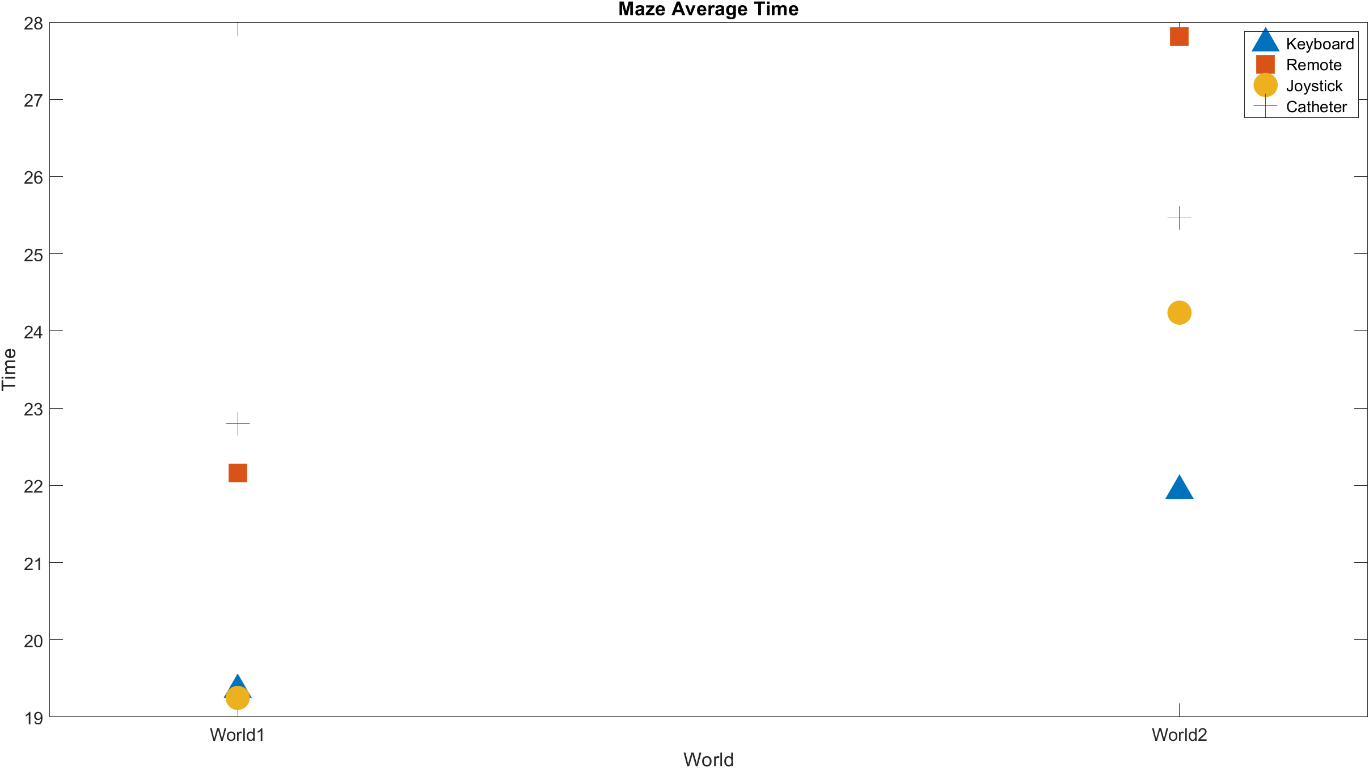
\includegraphics[width=1.0\textwidth]{img/maze/mazeAvgTime.png}
   \caption{Maze experiment average time per world}
   \label{img:mazeAvgTime}
\end{figure}

\begin{figure}[ht]
   \centering
   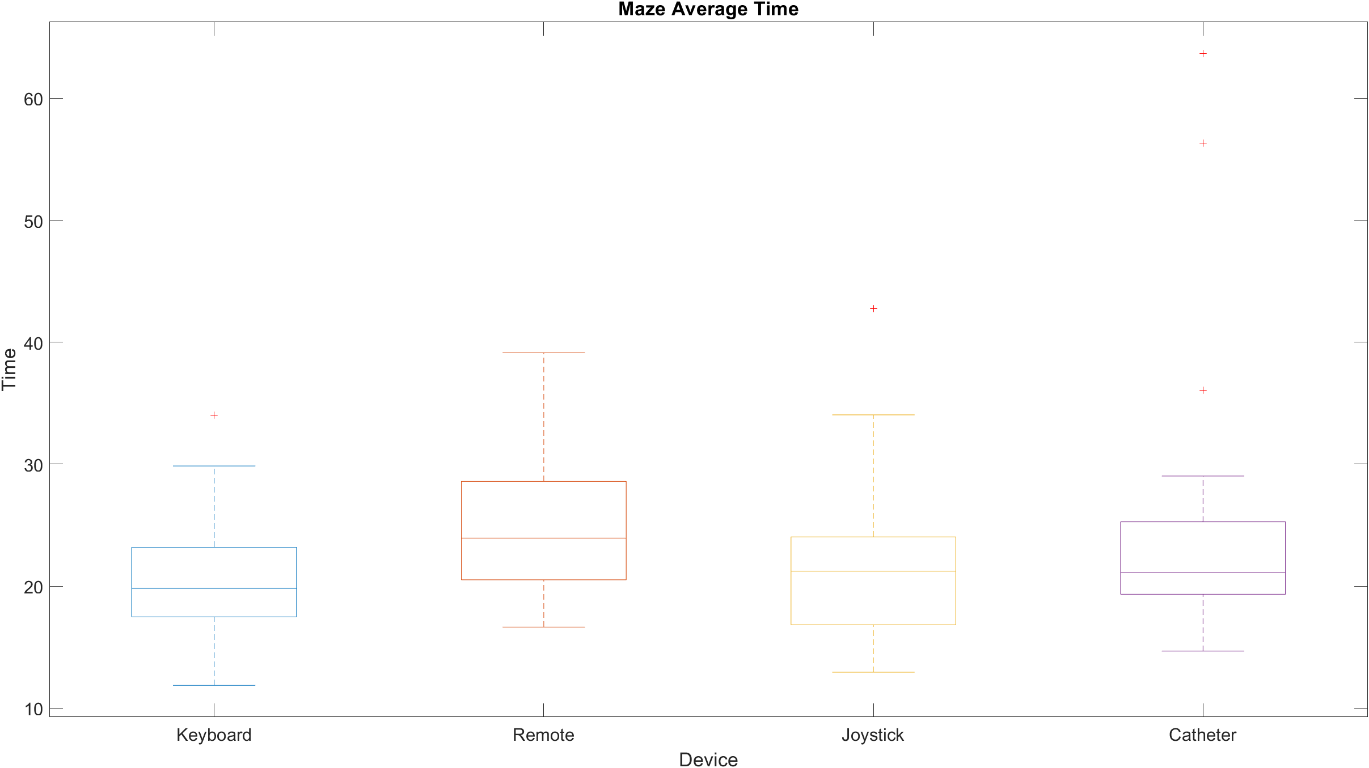
\includegraphics[width=1.0\textwidth]{img/maze/mazeTime.png}
   \caption{Maze experiment average time per device across all worlds}
   \label{img:mazeTime}
\end{figure}

\begin{figure}[ht]
   \centering
   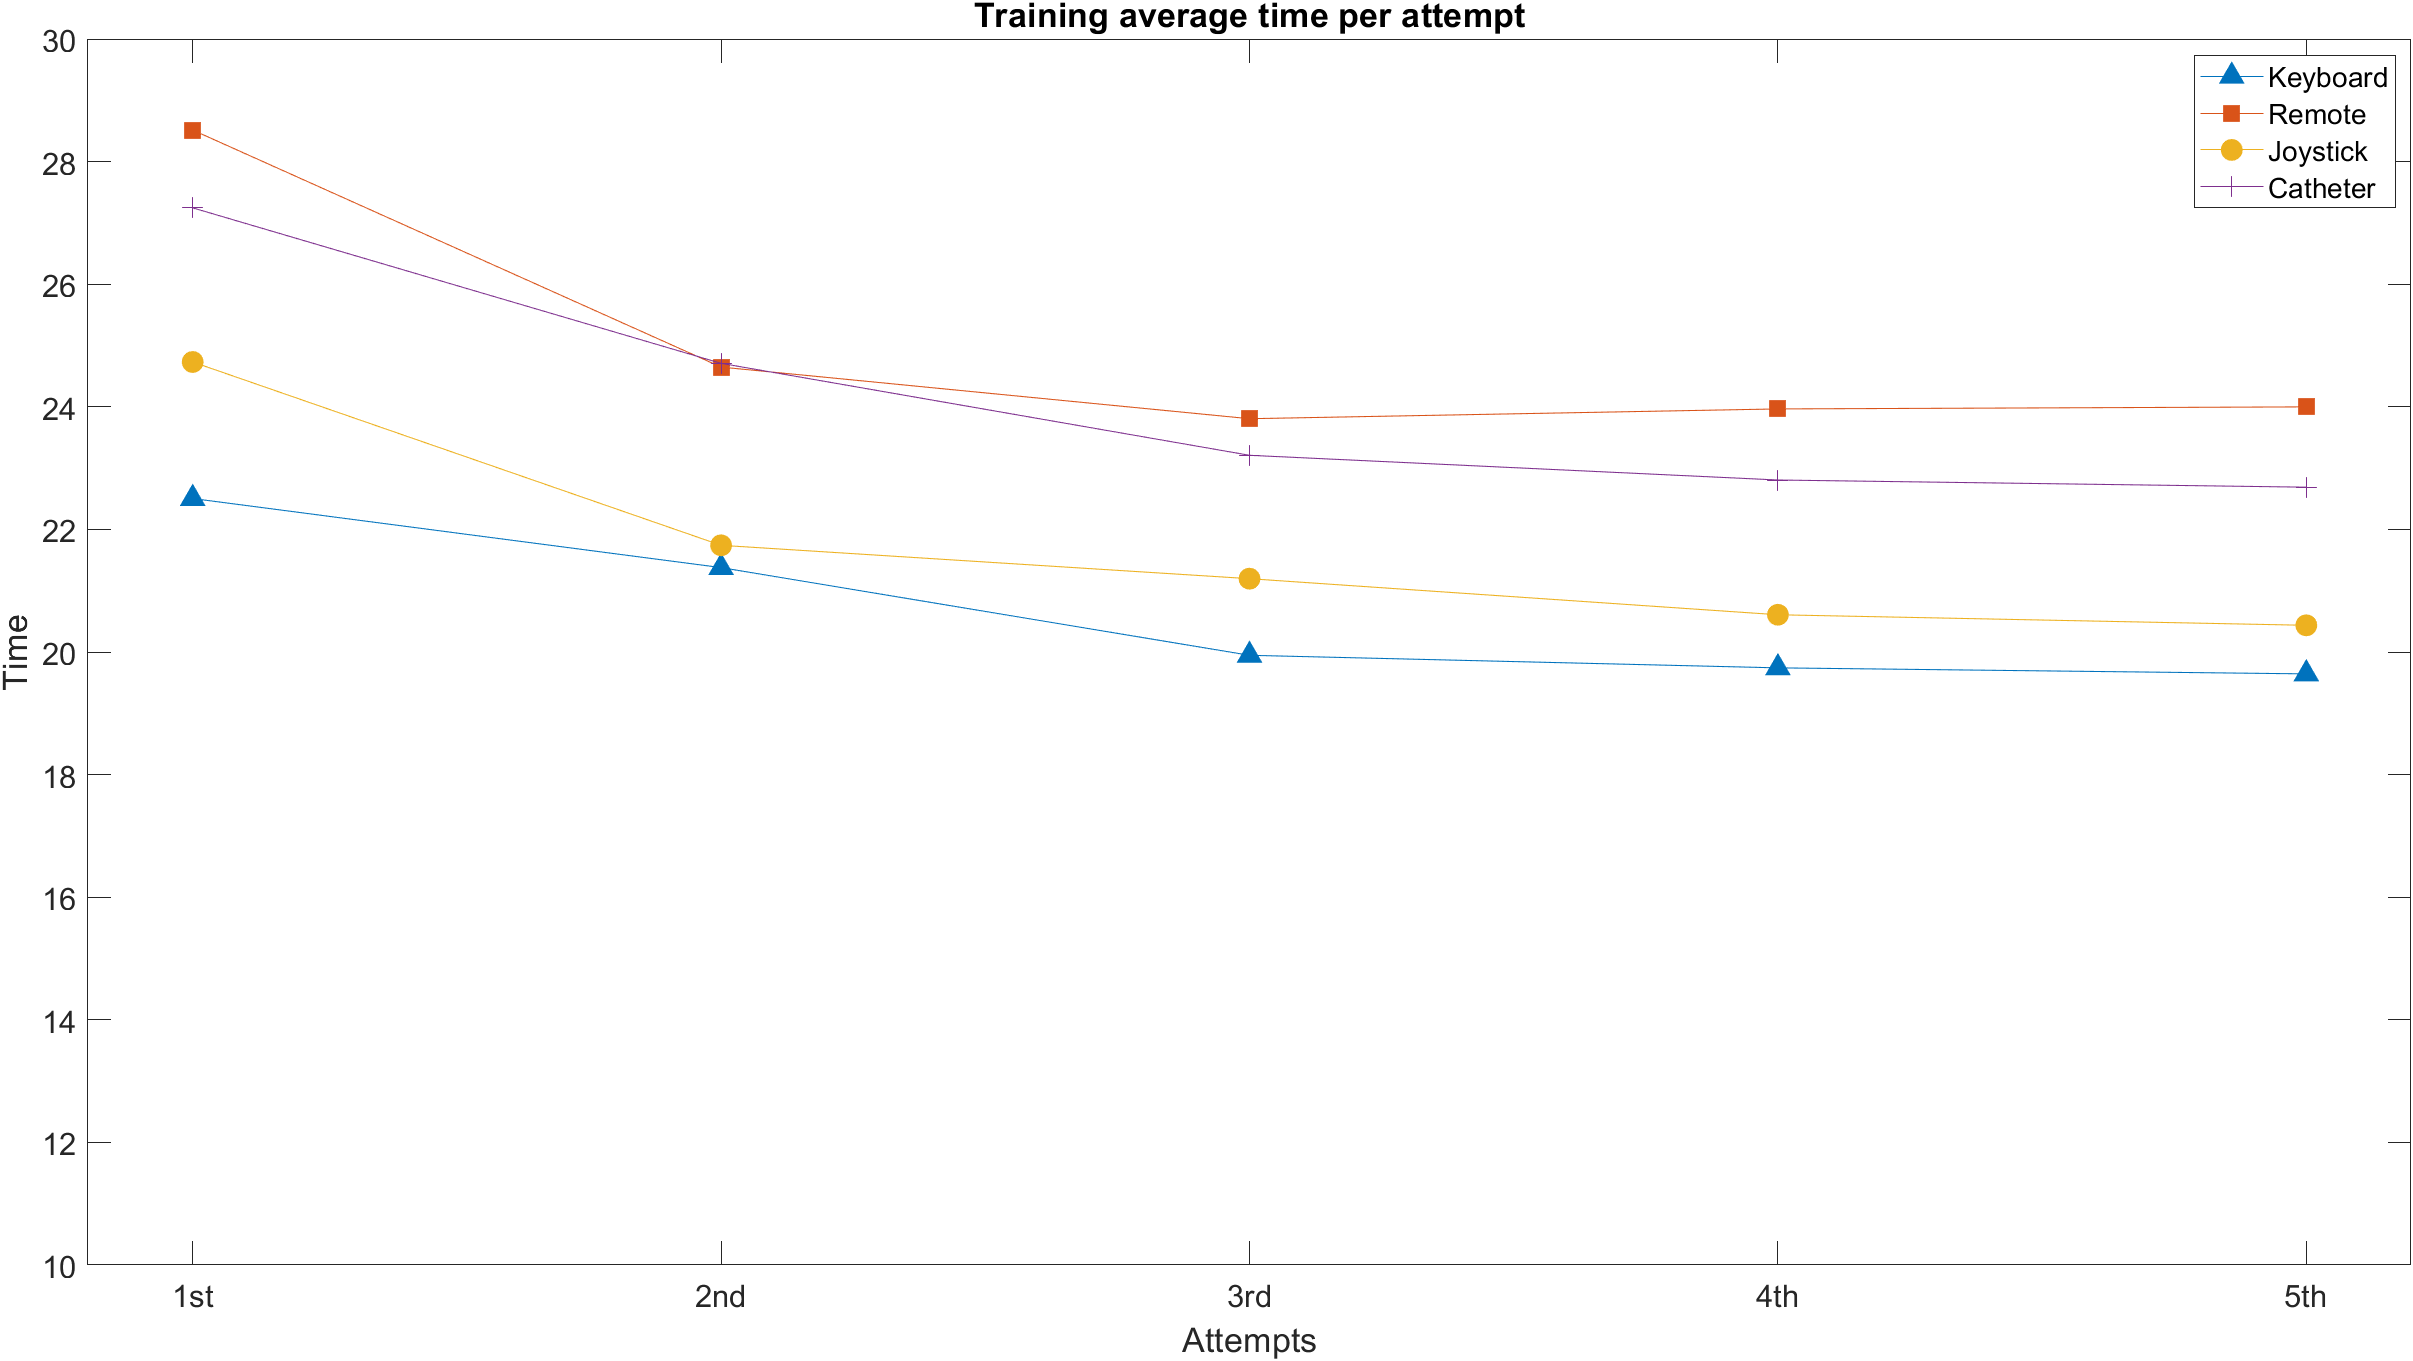
\includegraphics[width=1.0\textwidth]{img/maze/mazeTrainTime.png}
   \caption{Maze experiment time training curve of all participants}
   \label{img:mazeTrainTime}
\end{figure}

The average number of collisions (per repetition) shown in figure~\ref{img:mazeAvgColl} states that the Keyboard and Remote are significantly better than the Joystick and Catheter with a P-Value $<$ 0.01. This result gives again intuition about the importance of the advantages and disadvantages shown in figure~\ref{img:adtable}, if taking into account the information from figure~\ref{img:mazeAvgColl2}, where analogical sensor devices have a significantly higher amount of collisions in world2 (world with longer stretches) than in world1, combined with to the proneness of analogical sensor devices to overshot shows how important participants training is, and coming back to the Time results, it confirms how these collisions are related. This can be directly corroborated with the Joystick when putting together figure~\ref{img:mazeTrainColl} showing the collision training curve and figure~\ref{img:mazeTrainTime} showing the time training curve, where it can be appreciated how time per attempt goes down as collisions per attempt go down.\\

\begin{figure}[ht]
   \centering
   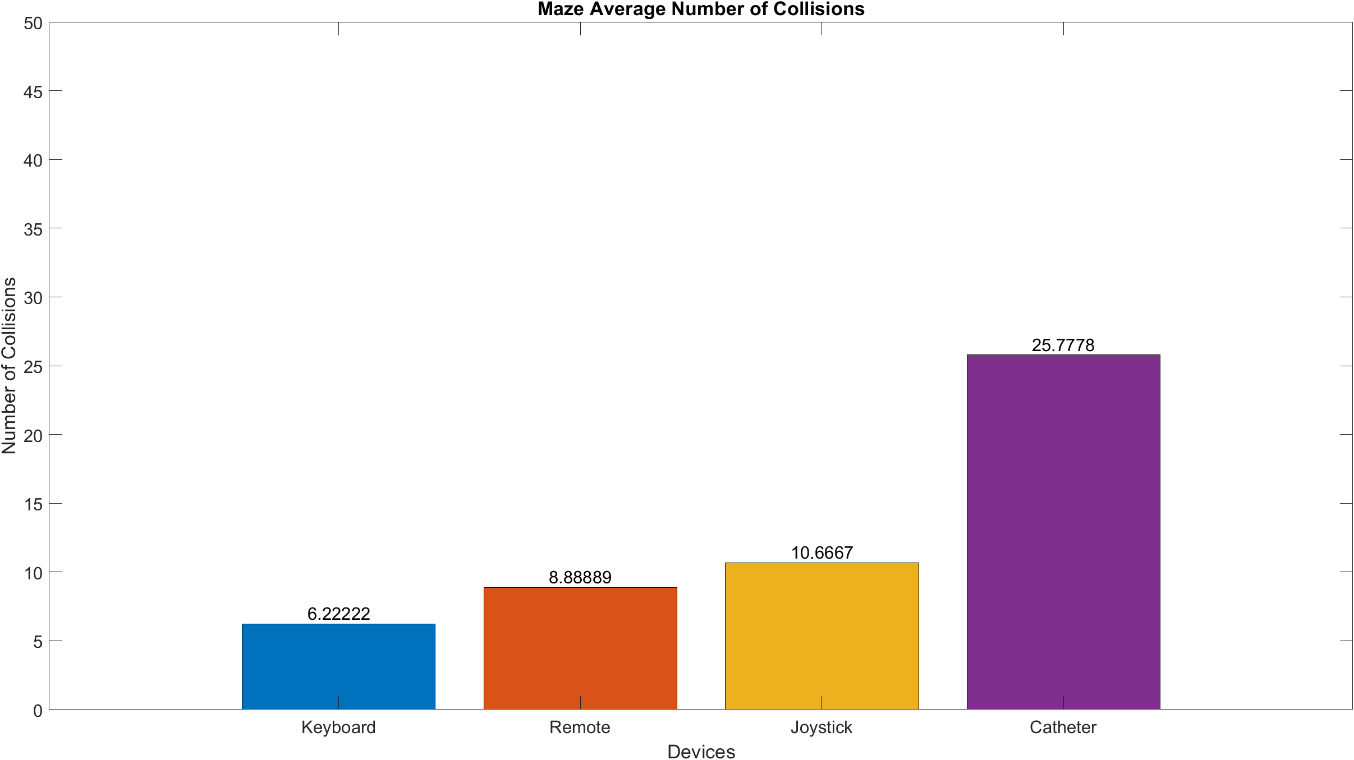
\includegraphics[width=1.0\textwidth]{img/maze/mazeAvgColl.png}
   \caption{Maze experiment average number of collisions per world}
   \label{img:mazeAvgColl}
\end{figure}

\begin{figure}[ht]
   \centering
   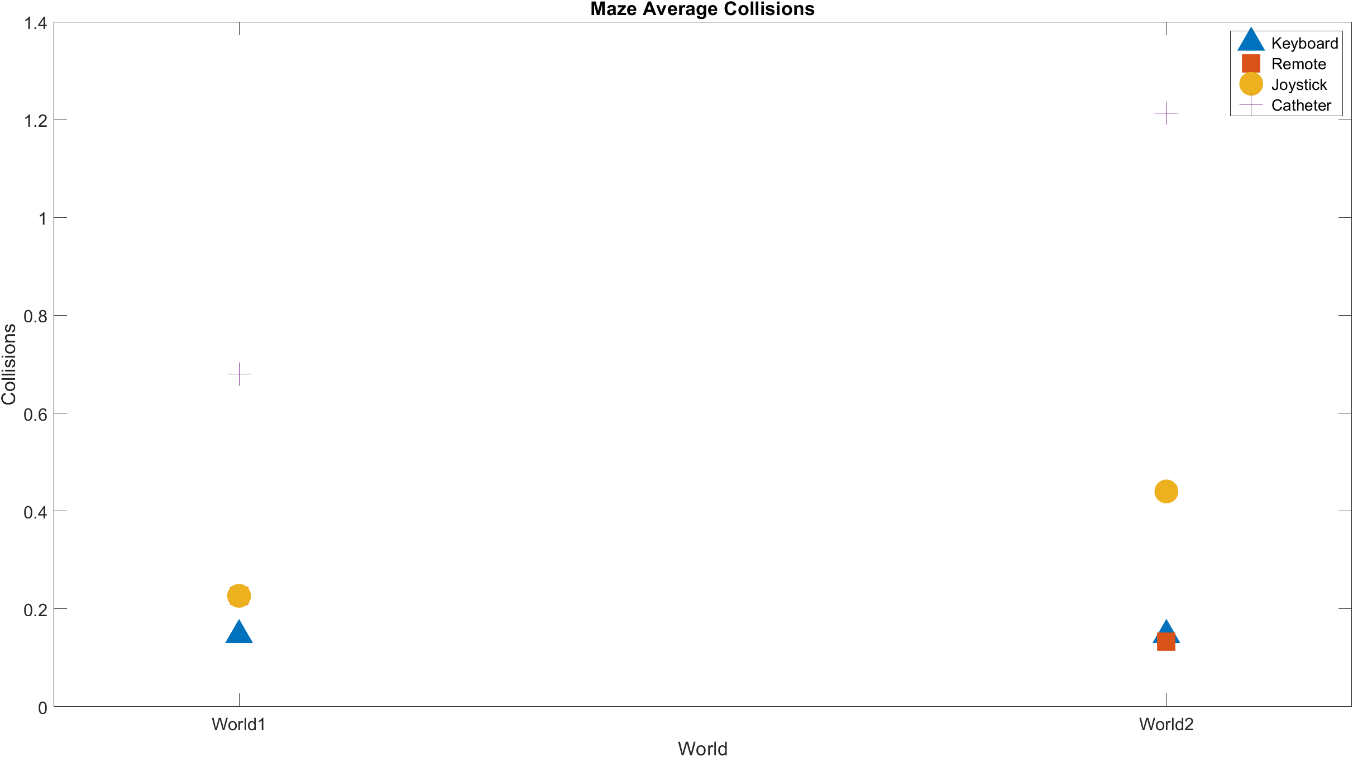
\includegraphics[width=1.0\textwidth]{img/maze/mazeAvgColl2.png}
   \caption{Maze experiment average number of collisions per device across all worlds}
   \label{img:mazeAvgColl2}
\end{figure}

\begin{figure}[ht]
   \centering
   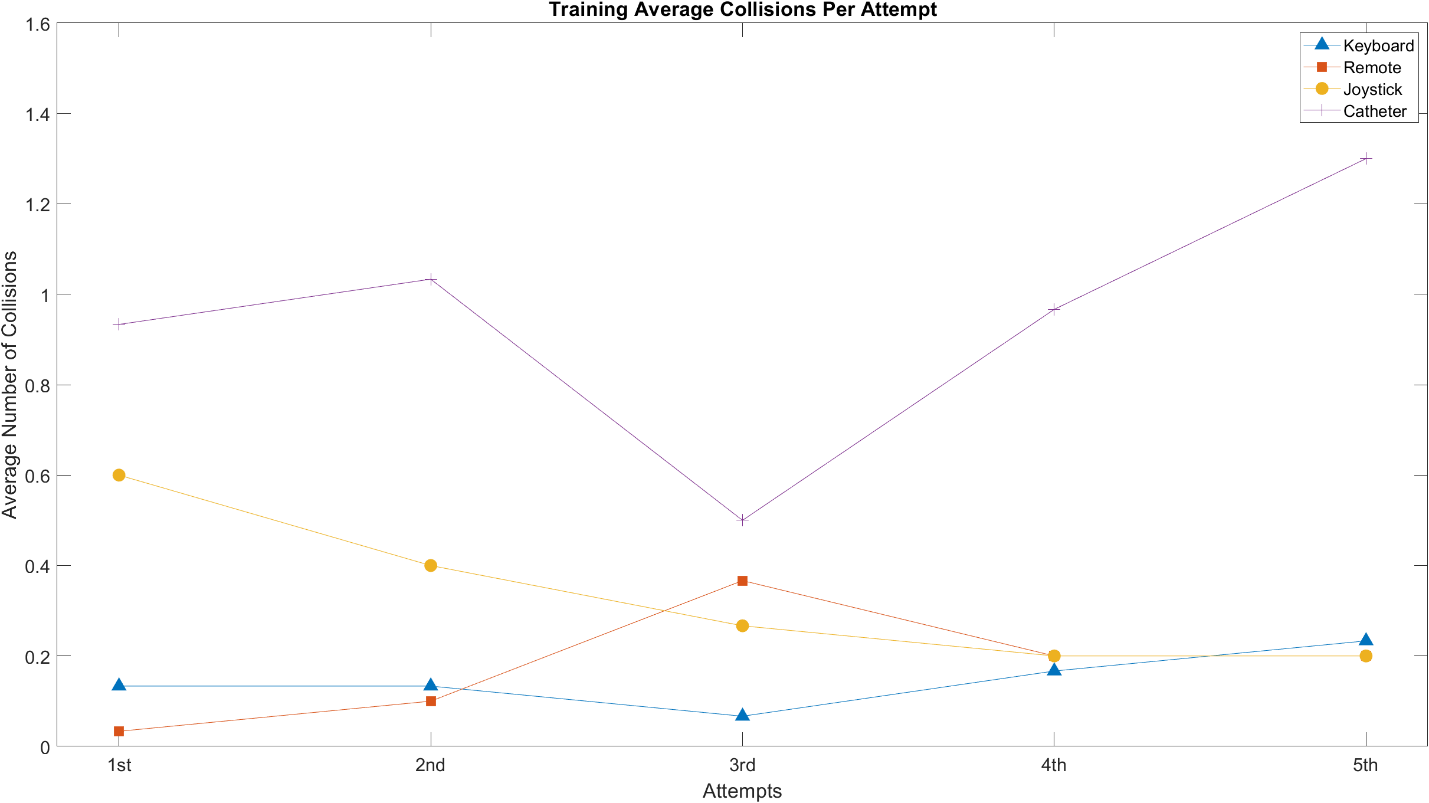
\includegraphics[width=1.0\textwidth]{img/maze/mazeTrainColl.png}
   \caption{Maze experiment number of collisions training curve of all participants}
   \label{img:mazeTrainColl}
\end{figure}

The joystick got a lower average Dimensionless Squared Jerk number in both worlds as shown in figure~\ref{img:mazeAvgDsj}, altough not significant due to an interaction P-Value lower than 0.05, immediatly followed by the keyboard device (figure~\ref{img:mazeDsj}). It is important to remark that part of the good result of the keyboard in the DSJ is due to the linear increment of thevelocity over time of the PressedTime-Velocity mapping; thus, if the function is changed to something non linear, this will have a high impact in this metric.\\

Also, it is important to remark how even though the Joystick had a worse performance than the keyboard in the collision average, and this collisions caused higher DSJ values, the performance overall in the DSJ was better. This may be due to the fact that the Keyboard can stop instantly, giving really high jerking values, which in a real world is also translated to high stress in the actuators.\\

\begin{figure}[ht]
   \centering
   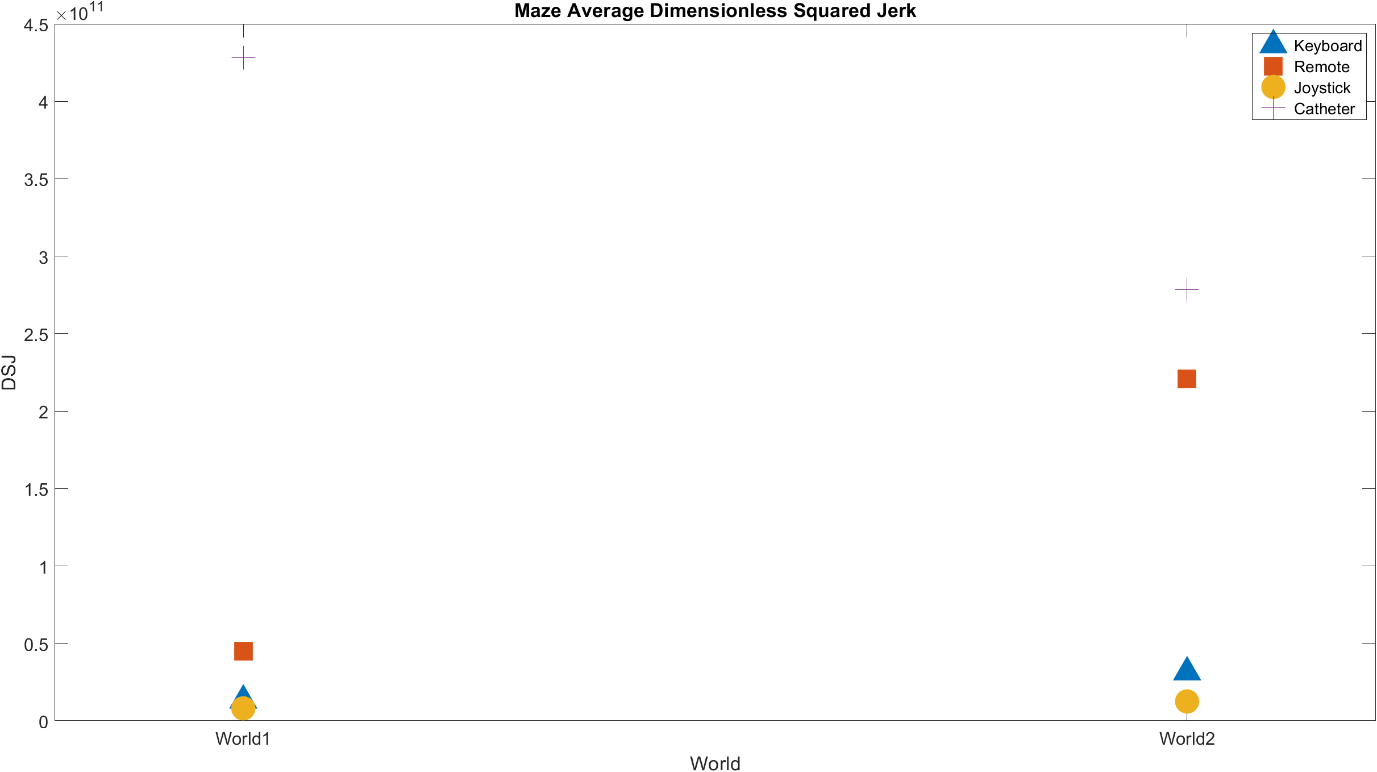
\includegraphics[width=1.0\textwidth]{img/maze/mazeAvgDsj.png}
   \caption{Maze experiment DSJ per world}
   \label{img:mazeAvgDsj}
\end{figure}

\begin{figure}[ht]
   \centering
   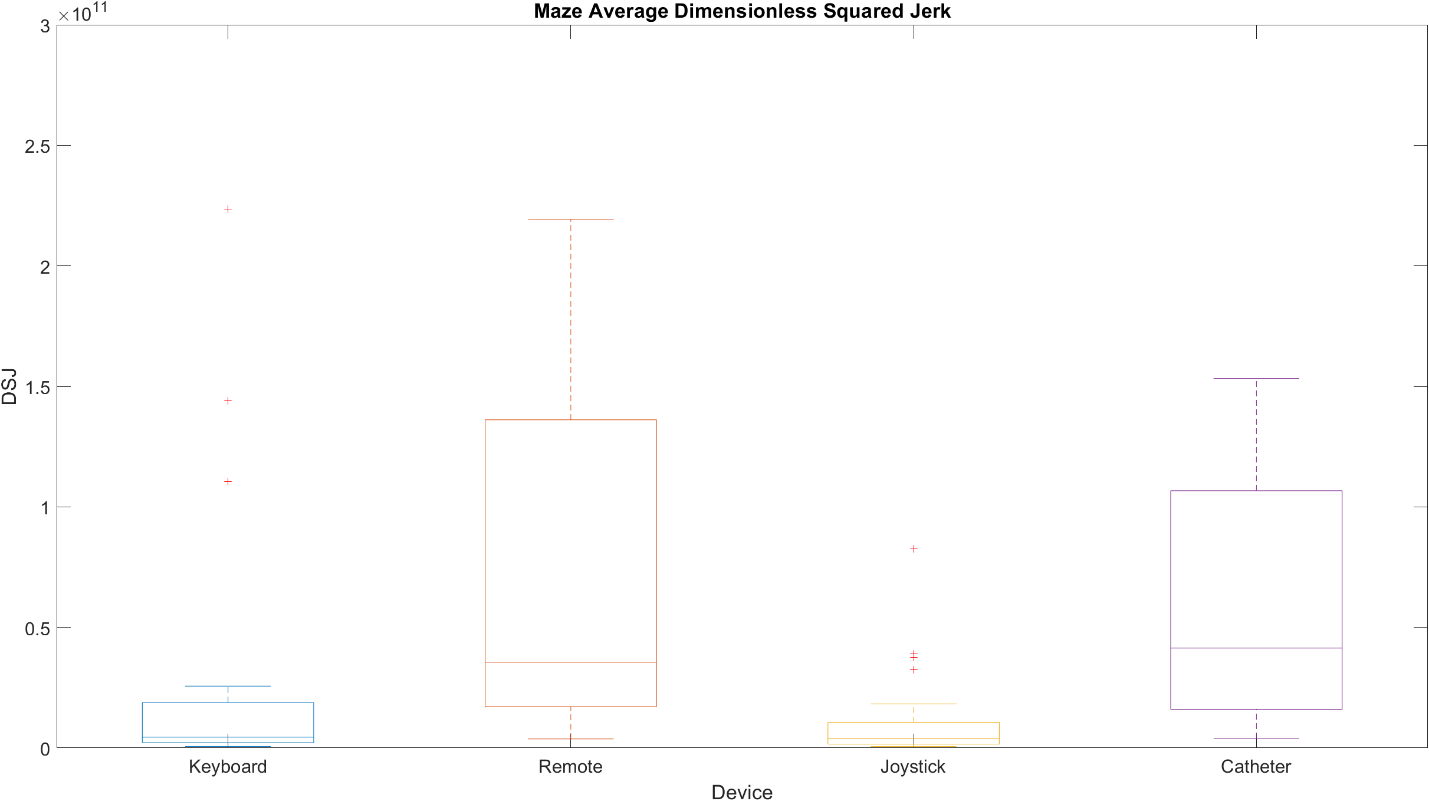
\includegraphics[width=1.0\textwidth]{img/maze/mazeDsj.png}
   \caption{Maze experiment DSJ per device across all worlds}
   \label{img:mazeDsj}
\end{figure}
\clearpage

\section{Poll Results}\label{sec:pollres}
After completing the experiment, each one of the participants were requested to answer questions about the performance of the devices and give any additional comments about the experiment/devices. The exact questions as they were handed to the participants can be found in appendix~\ref{sec:apsurv}.\\

Since the poll requested the participants to enumerate the preference for the devices from 1-4, the figure~\ref{img:1stpoll}, figure~\ref{img:2ndpoll} and figure~\ref{img:overallpoll}, were calculated as a percentage by adding all the points each device got and dividing by the total amount of points. It can be seen for the 1st DOF device preference, the Joystick has the higher punctuation, followed by the Keyboard and then the Remote, leaving the CatheterLike last. Moreover, the 2nd DOF has in first place the Joystick again, in this case followed by the remote, then the Keyboard and last the CatheterLike device. The overall poll had the same results as in the 1st DOF, but note that the difference between keyboard and remote was significantly reduced.\\

Another one of the questions asked to the participants was the experience with the devices, shown in figure~\ref{img:expdev}, which shows how many participants out of the 15 declared experience in any of the devices, with the Keyboard being the most used, followed by the Joystick.\\

The most relevant comments made by the participants are as follow:
\begin{itemize}
 \item  Remote appears to be significantly slower than keyboard in the 1st DOF
 \item Takes some time to operate the joystick, but with time it feels the easiest to use
 \item Rotation in joystick has too much dead zone and no low velocity
 \item 	(From Surgeon) The final user interface could use the Joystick as main device and the Remote as detachable device for being able to operate near the patient if necessary.\\
\end{itemize}

\begin{figure}[ht]
   \centering
   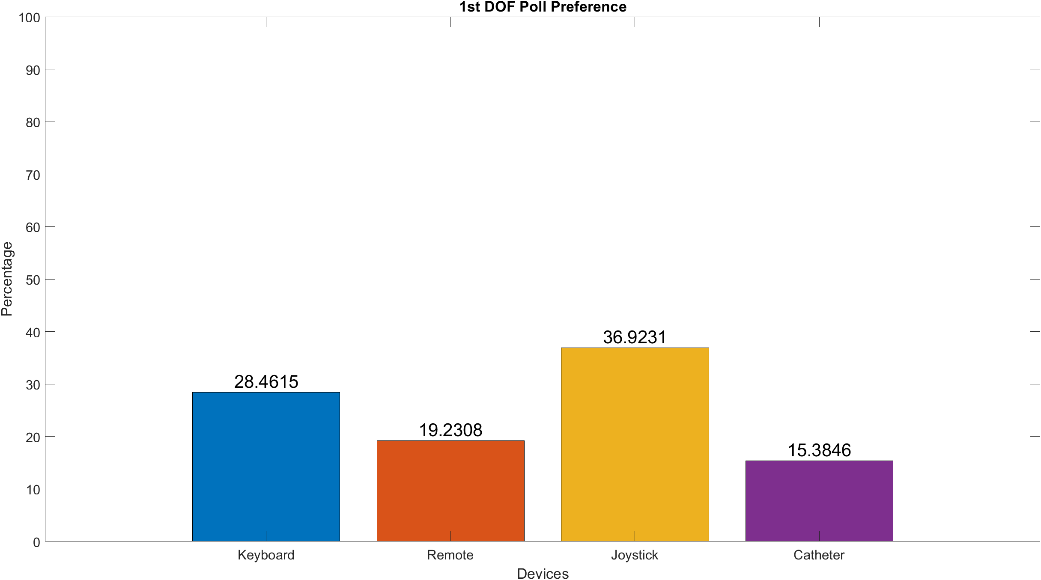
\includegraphics[width=1.0\textwidth]{img/poll/1stpoll.png}
   \caption{Participants percentage of preference per device on the 1st DOF}
   \label{img:1stpoll}
\end{figure}

\begin{figure}[ht]
   \centering
   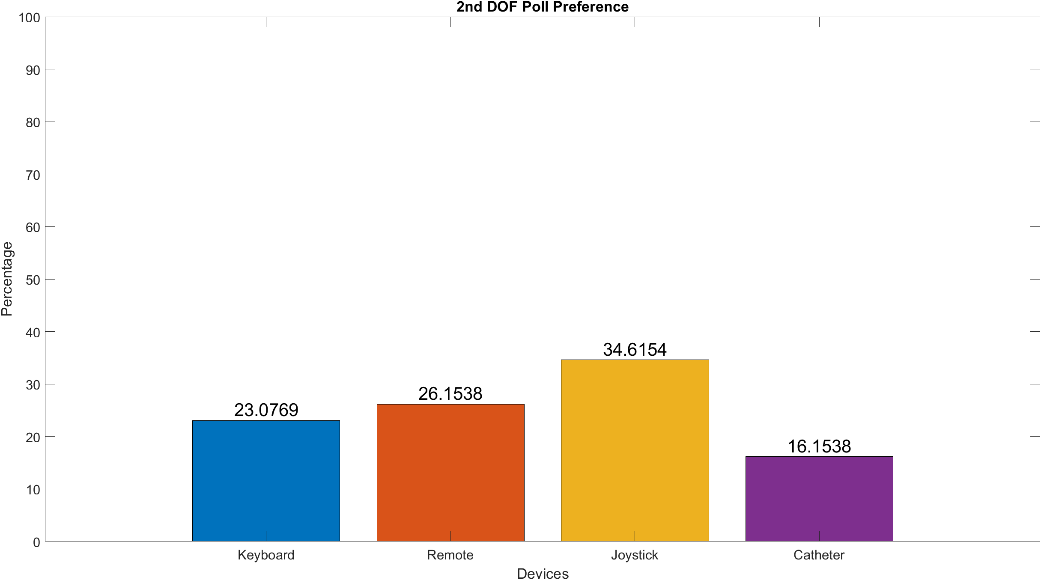
\includegraphics[width=1.0\textwidth]{img/poll/2ndpoll.png}
   \caption{Participants percentage of preference per device on the 2nd DOF}
   \label{img:2ndpoll}
\end{figure}

\begin{figure}[ht]
   \centering
   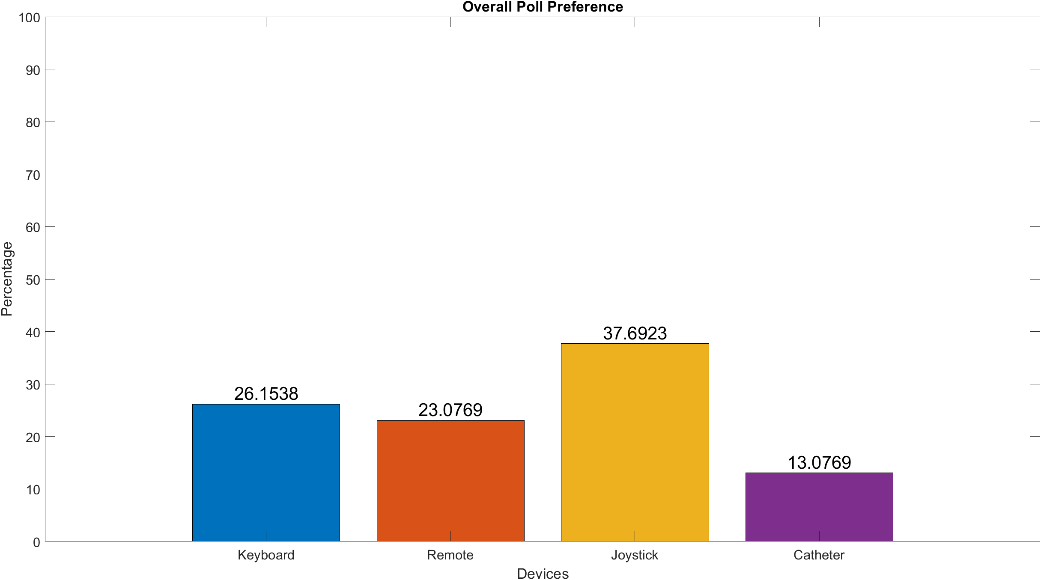
\includegraphics[width=1.0\textwidth]{img/poll/overallpoll.png}
   \caption{Participants percentage of preference per device on the overall}
   \label{img:overallpoll}
\end{figure}

\begin{figure}[ht]
   \centering
   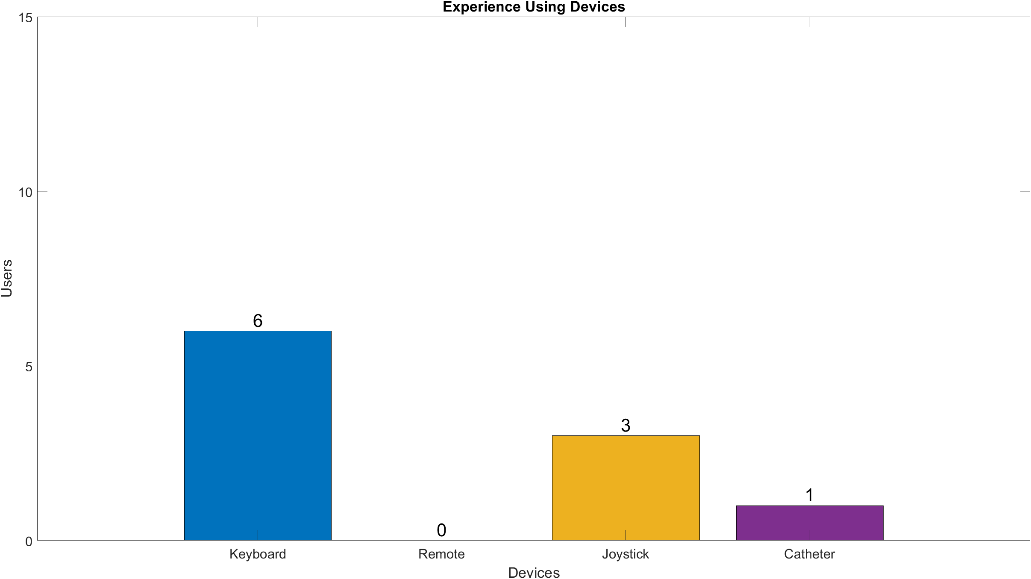
\includegraphics[width=1.0\textwidth]{img/poll/expdev.png}
   \caption{Number of participants with experience with each master device}
   \label{img:expdev}
\end{figure}



\cleardoublepage
% ...
% \input{}
% \cleardoublepage
% \input{}b
% \cleardoublepage
% ...
% !TeX root = /../Report.tex

\chapter{Conclusion}\label{chap:conclusion}


\section{Summary} \label{summary}


\section{Conclusion} \label{conclusion}


\section{Future work} \label{futurework}

\cleardoublepage

% Appendix______________________________________________________________________
\appendix
% !TeX root = /../Report.tex

\chapter{Something}\label{sec:something}

Put things for completeness here, to which you refer, but which are not part of the grading.
E.g. Reference tables, source code examples \dots

 \cleardoublepage


\chapter{Again Something}\label{sec:again_something}

Blah, blah \dots

 \cleardoublepage



% Bibliography__________________________________________________________________
% Literature (Additional references can be added to the .bib-file manually, or by using, for example, the free application JabRef). Compile in the following order: latex -bibtex -latex -latex

%Bibliographie
%bibliography
\bibliographystyle{plain}
\bibliography{bibliography}
\cleardoublepage

\end{document}